%*************************************
% บทที่ 3
%*************************************
\chapterTitle{3}{วิธีการดำเนินงานและการออกแบบระบบ}

\section{การออกแบบสถาปัตยกรรมระบบ}

\subsection{สถาปัตยกรรมระบบโดยรวม}

\hspace*{1.3em} %ย่อหน้า
ระบบแพลตฟอร์มคลัสเตอร์เสมือนในฉบับพัฒนาปัจจุบันยังคงยึดแนวคิด Microservices Architecture แต่เมื่อพิจารณาทั้งบริการหลักและบริการสนับสนุนที่ใช้ในการติดตั้งจริง สามารถแบ่งองค์ประกอบออกเป็น 5 บทบาทสำคัญ คือ
\begin{mycustomitem}
    \item \textbf{Frontend (Midori)} เว็บแอปพลิเคชันสำหรับผู้ใช้งาน พัฒนาด้วย Next.js และ React ทำหน้าที่เป็นส่วนติดต่อผู้ใช้สำหรับนักศึกษา อาจารย์ และผู้ดูแลระบบ
    \item \textbf{API Service (Momoi)} เซิร์ฟเวอร์หลักของระบบ พัฒนาด้วย Bun, Elysia.js และ Prisma รับผิดชอบโดเมนด้านข้อมูลวิชาการ คำร้องขอเครื่องเสมือน การจัดการเครื่องเสมือน พื้นที่จัดเก็บไฟล์ การยืนยันตัวตนผ่านเส้นทาง `/api/auth` และการเชื่อมต่อกับบริการภายนอก
    \item \textbf{Worker / VM Management (Yuzu)} เซอร์วิสประมวลผลงานเบื้องหลังสำหรับการสร้าง ลบ และเปลี่ยนสถานะเครื่องเสมือน โดยสื่อสารกับ Proxmox VE แบบ Asynchronous
    \item \textbf{Reverse Proxy and Access Automation (Satsuki)} บริการที่ติดตั้งบนเครื่อง Nginx ภายนอกซึ่งทำหน้าที่เป็น reverse proxy หน้าด่านของระบบ ใช้สร้างไฟล์ reverse proxy configuration และ `authorized\_keys` จากข้อมูลในฐานข้อมูล พร้อมติดตามการเปลี่ยนแปลงด้วย PostgreSQL LISTEN/NOTIFY และสั่ง reload บริการปลายทางเมื่อข้อมูลเปลี่ยน
    \item \textbf{Supporting Services and Deployment (Yuuka)} ชุดโครงสร้างพื้นฐานและไฟล์สำหรับการติดตั้งใช้งานจริง เช่น PostgreSQL, Redis, RustFS และระบบสังเกตการณ์การทำงานของแพลตฟอร์ม
\end{mycustomitem}

\hspace*{1.3em} %ย่อหน้า
ในสภาพแวดล้อมที่ติดตั้งใช้งานจริง เส้นทางการทำงานหลักของระบบสามารถสรุปได้เป็น Browser > Midori > Momoi สำหรับคำขอด้านข้อมูล ตรรกะทางธุรกิจ และการยืนยันตัวตนผ่าน `/api/auth` ส่วนงานที่ใช้เวลานาน เช่น การสร้าง ลบ หรือเปลี่ยนสถานะเครื่องเสมือน จะถูก Momoi ส่งเข้าสู่ Redis-backed BullMQ ก่อนที่ Yuzu จะรับงานไปดำเนินการกับ Proxmox VE ต่อไป และเมื่อข้อมูล reverse proxy หรือ SSH key เปลี่ยนแปลง Satsuki ซึ่งทำงานอยู่บนเครื่อง Nginx ภายนอกจะรับสัญญาณจากฐานข้อมูลเพื่อสร้างไฟล์กำหนดค่าที่เกี่ยวข้องใหม่และ reload reverse proxy หน้าด่านโดยอัตโนมัติ การแยกเส้นทางแบบนี้ทำให้ระบบส่วนติดต่อผู้ใช้และ API ตอบสนองได้รวดเร็ว แม้งานด้านโครงสร้างพื้นฐานจะมีระยะเวลาดำเนินการยาวนานกว่ามาก

\begin{figure}[H]
    \centering
    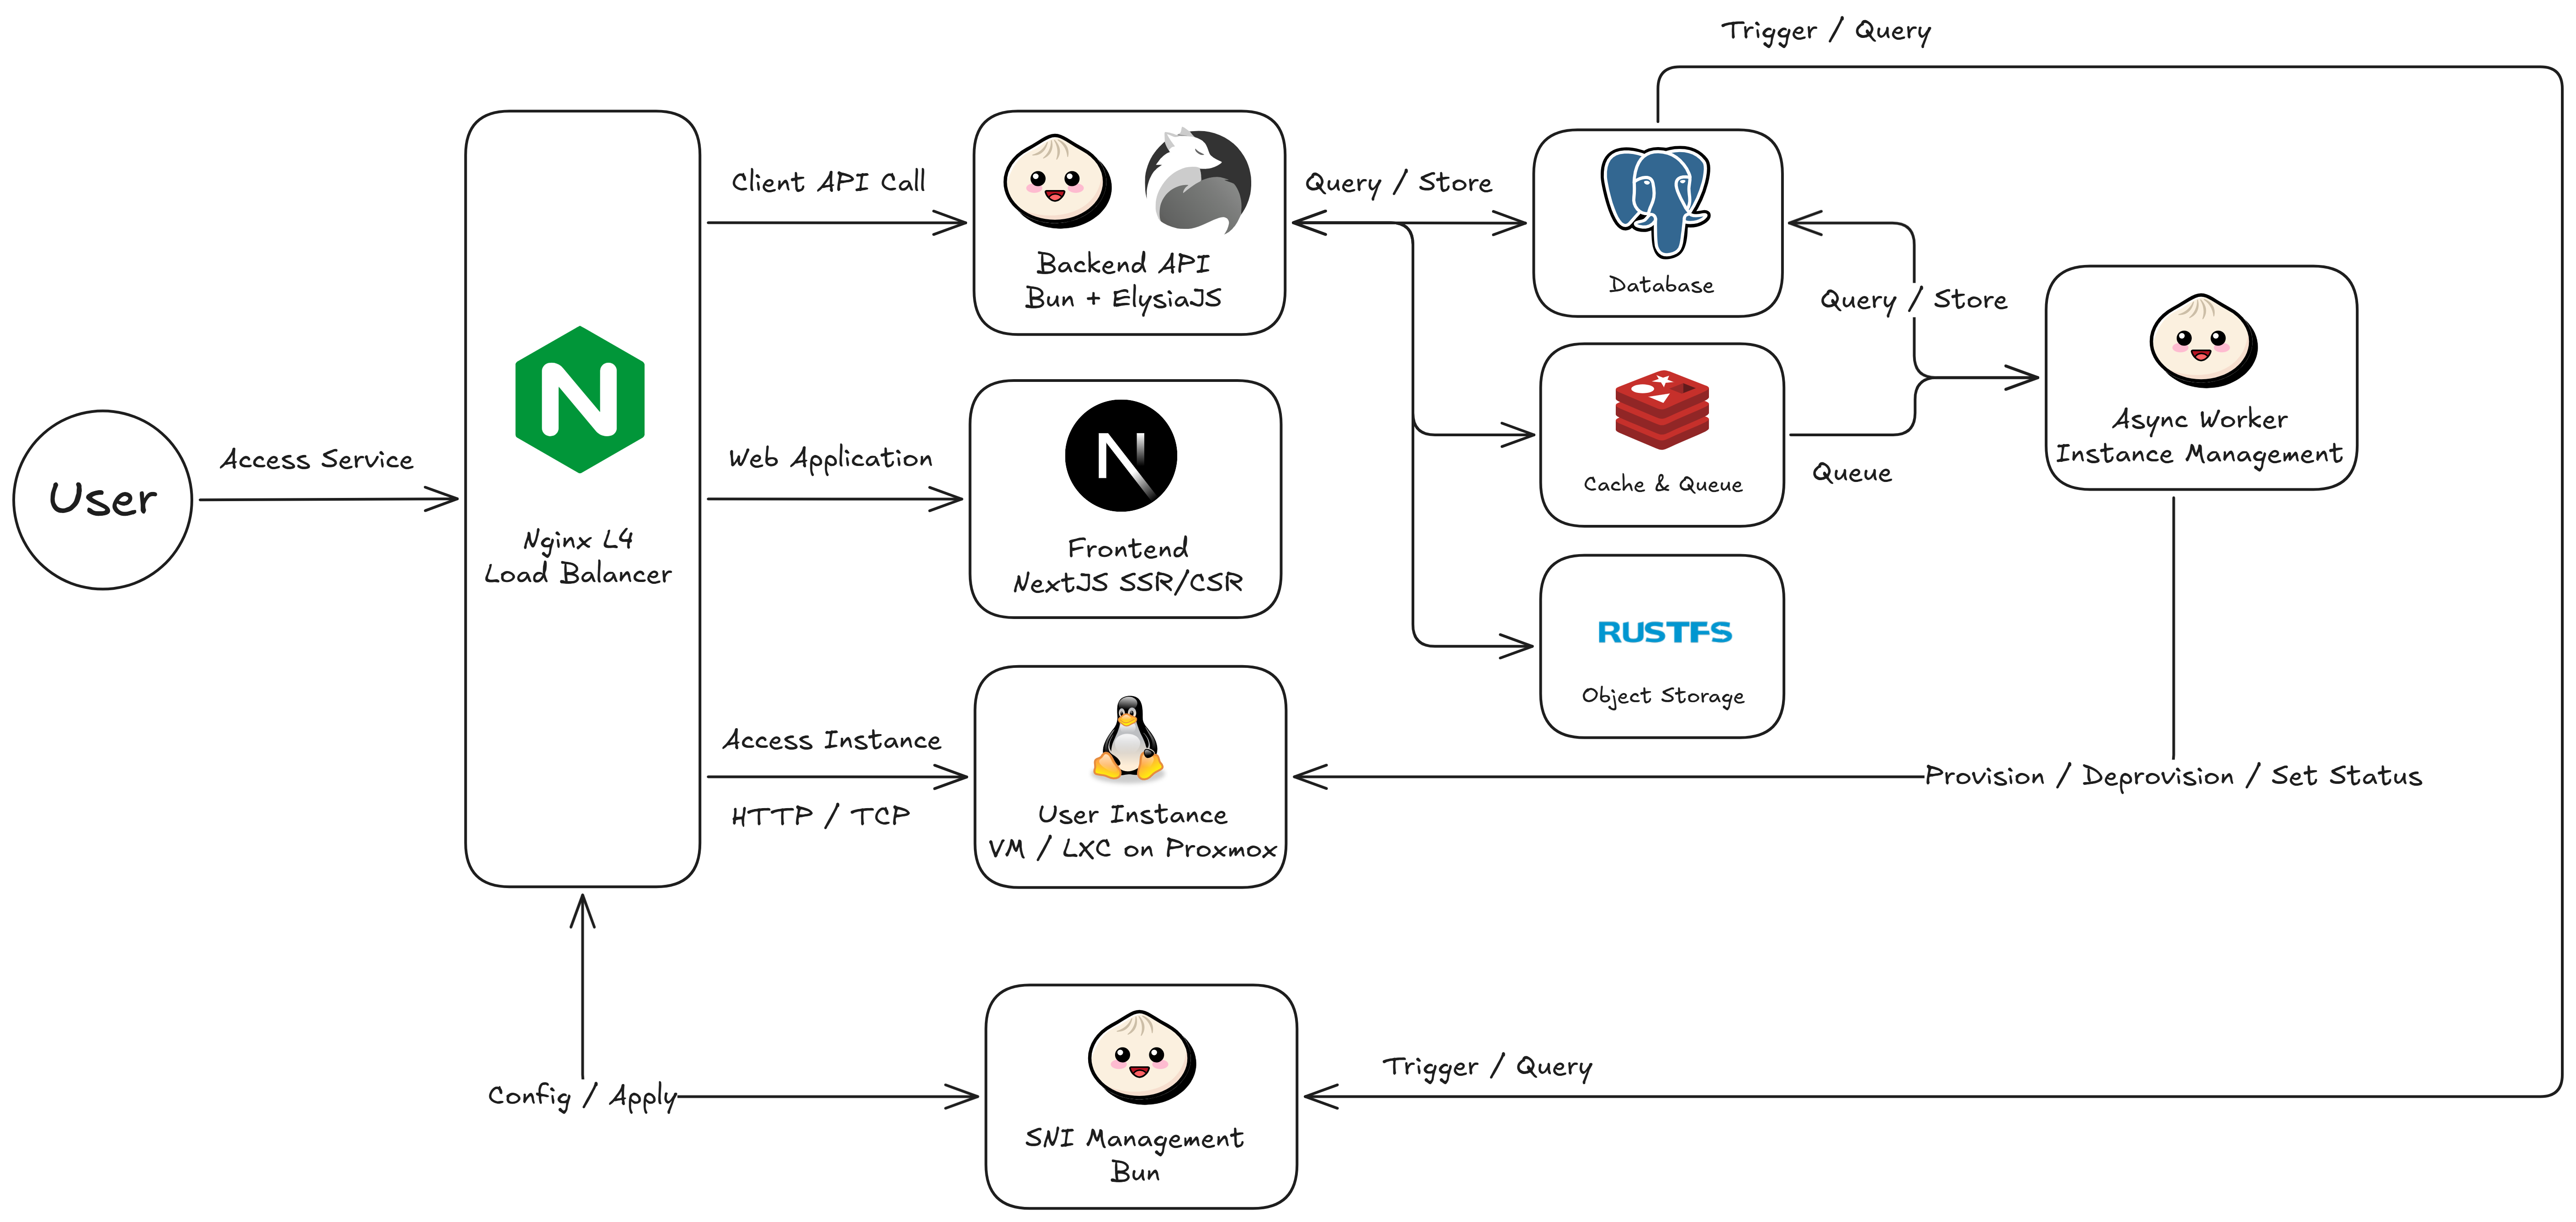
\includegraphics[width=1.0\linewidth]{Image/current_system_diagram.png}
    \caption{\fontSixTeen{แผนภาพการทํางานและลําดับขั้นตอนโดยรวมของโปรแกรม}}
    \label{fig3:system_overview_flow}
\end{figure}

\hspace*{1.3em} %ย่อหน้า
จากภาพที่ \ref{fig3:system_overview_flow} จะเห็นลำดับการทำงานหลักของแพลตฟอร์มอย่างเป็นขั้นตอน โดยผู้ใช้เริ่มต้นจากการเข้าใช้งานผ่าน Midori ซึ่งเป็นส่วนติดต่อผู้ใช้ จากนั้นคำขอจะถูกส่งต่อไปยัง Momoi เพื่อประมวลผลตรรกะทางธุรกิจ ตรวจสอบสิทธิ์ และบันทึกข้อมูลลงในฐานข้อมูล หากเป็นงานที่ต้องใช้เวลานานหรือเกี่ยวข้องกับการจัดสรรทรัพยากรเครื่องเสมือน Momoi จะส่งงานเข้าสู่คิวเพื่อให้ Yuzu รับไปดำเนินการกับ Proxmox VE แบบอะซิงโครนัส ขณะเดียวกันข้อมูลที่เกี่ยวข้องกับ reverse proxy และ SSH access จะถูก Satsuki ซึ่งติดตั้งอยู่บนเครื่อง Nginx ภายนอกนำไปสร้างไฟล์กำหนดค่าและ reload บริการหน้าด่านให้สอดคล้องกับสถานะล่าสุดของระบบ ภาพนี้จึงช่วยสรุปความสัมพันธ์ระหว่างบริการหลัก เส้นทางข้อมูล และจุดที่เกิดการประมวลผลเบื้องหลัง ก่อนจะลงรายละเอียดในแผนภาพบริบทและแผนภาพการไหลของข้อมูลระดับถัดไป

% แผนภาพนี้ควรรีเจนจากไฟล์ Mermaid: docs/diagram/chapter3-context-diagram.mmd
\begin{figure}[H]
    \centering
    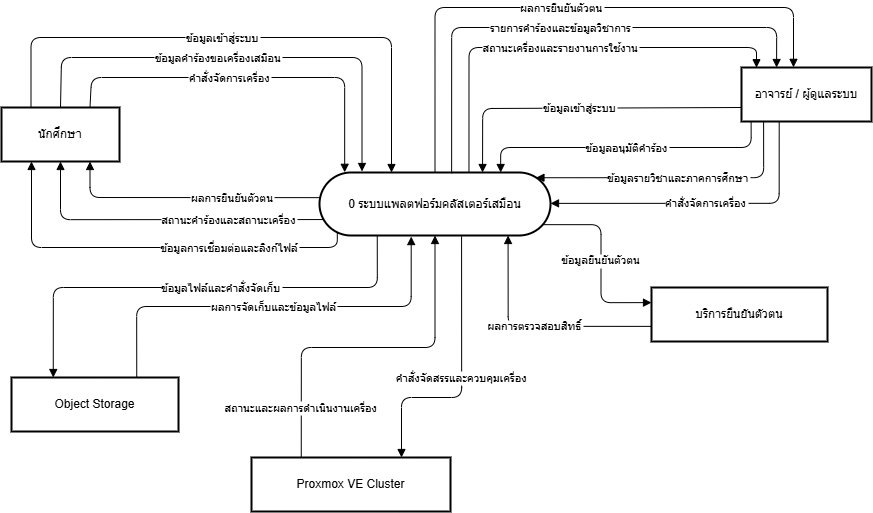
\includegraphics[width=1.0\linewidth]{Image/diagram/chapter3-context-diagram.png}
    \caption{\fontSixTeen{แผนภาพบริบทของระบบแพลตฟอร์มคลัสเตอร์เสมือน}}
    \label{fig3:context_diagram}
\end{figure}

\hspace*{1.3em} %ย่อหน้า
จากภาพที่ \ref{fig3:context_diagram} ระบบถูกมองเป็นกระบวนการเดียวในลักษณะ Black Box เพื่อแสดงเฉพาะความสัมพันธ์ระหว่างระบบกับเอนทิตีภายนอก ได้แก่ นักศึกษา อาจารย์หรือผู้ดูแลระบบ บริการยืนยันตัวตน Proxmox VE Cluster และ Object Storage โดยไม่มีการแสดงแหล่งเก็บข้อมูลภายในตามหลักของ Context Diagram จากนั้นในภาพที่ \ref{fig3:data_flow_level_0} ได้ทำการแตกกระบวนการหลักของระบบออกเป็น 5 กระบวนการ พร้อมเพิ่มแหล่งเก็บข้อมูลที่จำเป็น โดยแยกแสดงเป็น 3 มุมมองเพื่อความชัดเจน และในภาพที่ \ref{fig3:data_flow_level_1_auth} – \ref{fig3:data_flow_level_1_vm} ได้ขยายรายละเอียดทั้ง 5 กระบวนการหลัก เพื่อรักษาความสมดุลของกระแสข้อมูลระหว่างแต่ละระดับของ DFD ให้สอดคล้องกัน

% แผนภาพนี้ควรรีเจนจากไฟล์ Mermaid: docs/diagram/chapter3-dataflow-level0.mmd
\begin{figure}[H]
    \centering
    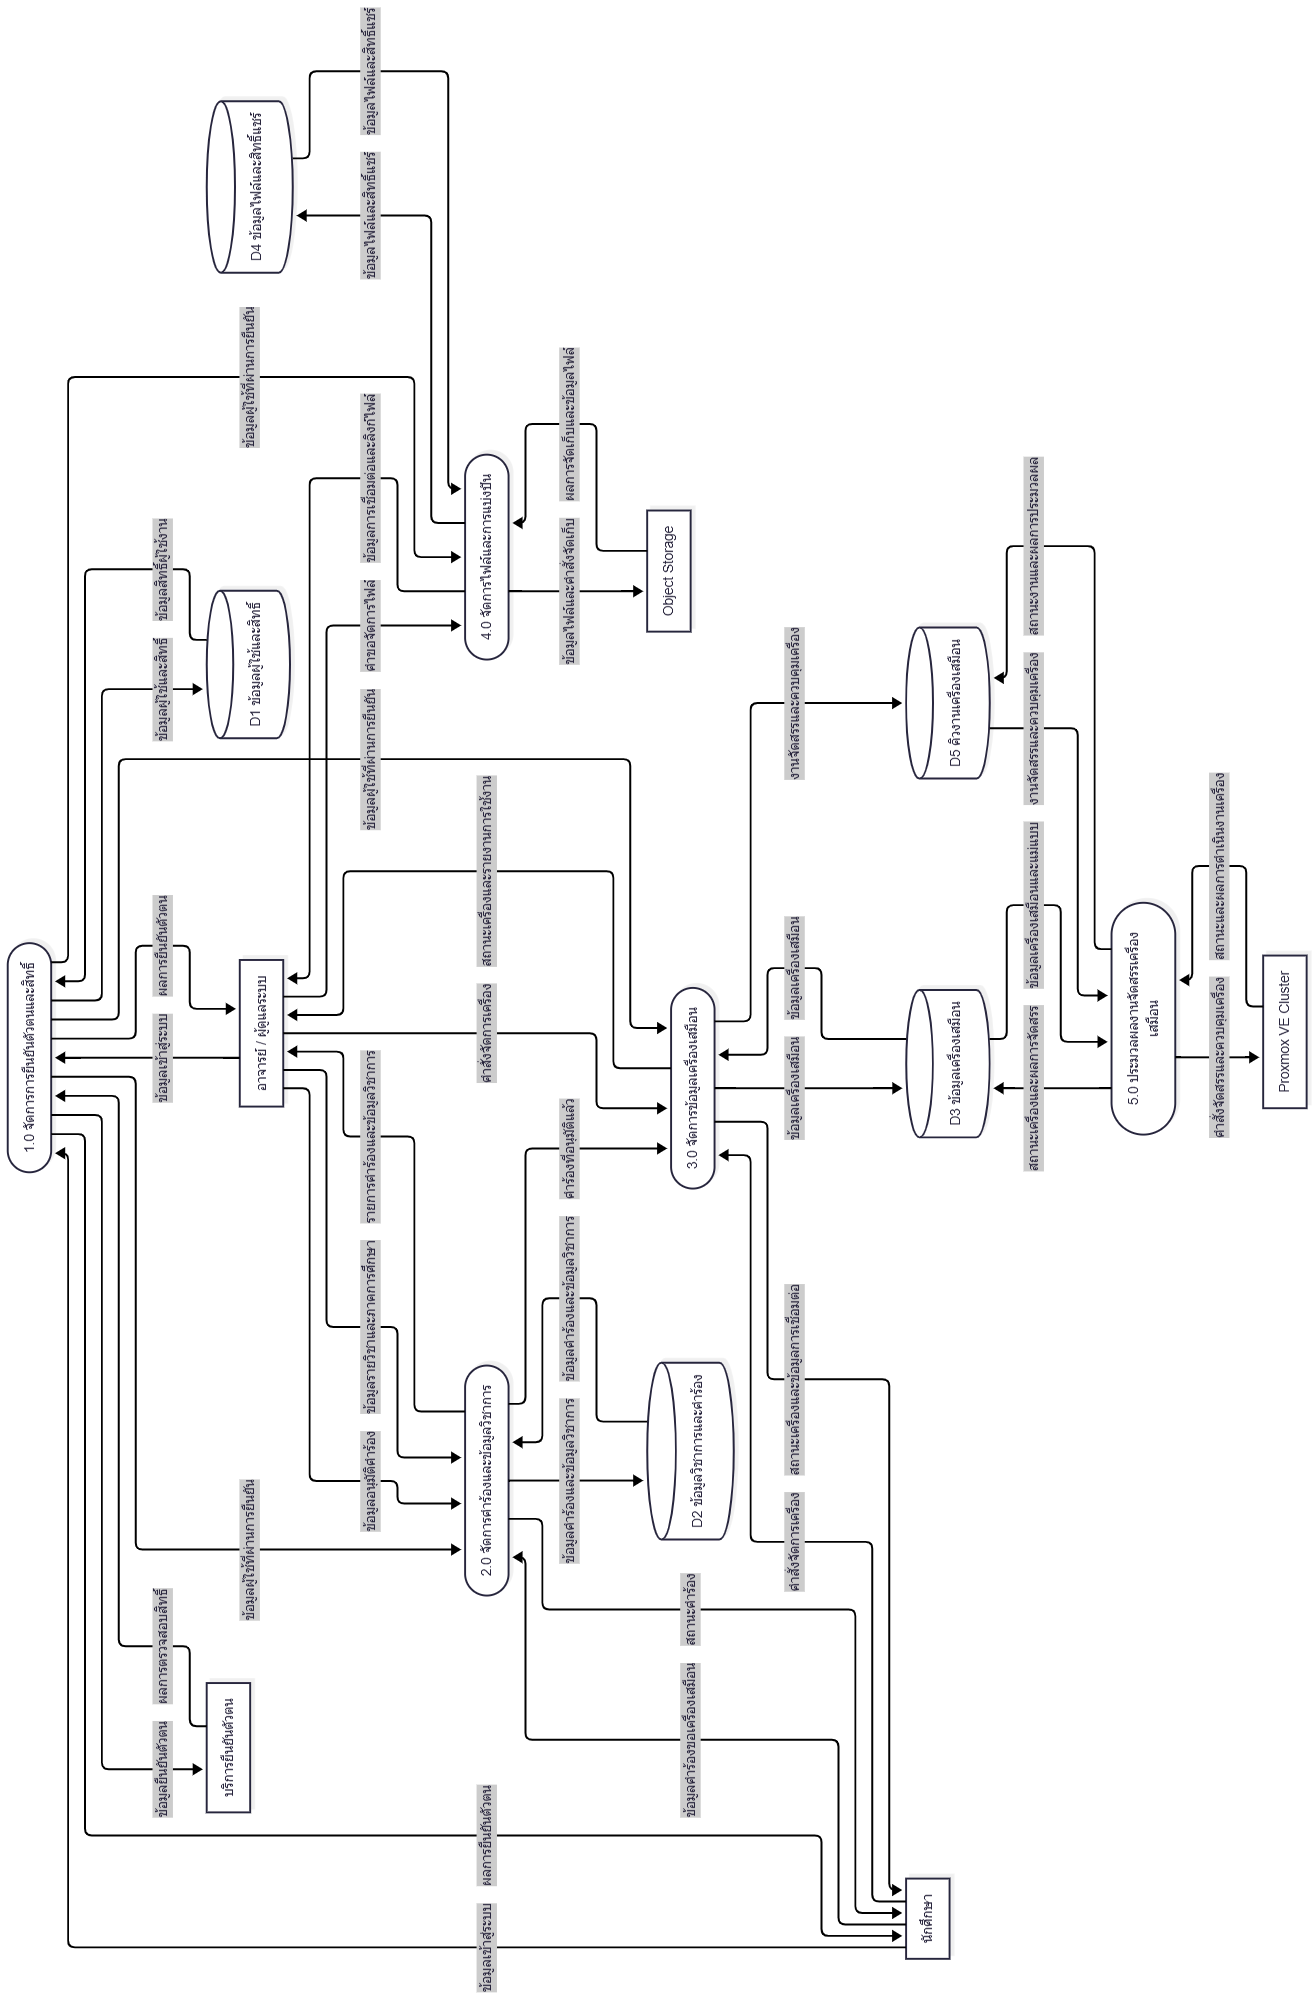
\includegraphics[width=1.0\textwidth]{Image/diagram/chapter3-dataflow-level0_90.png}
    \caption{\fontSixTeen{แผนภาพการไหลของข้อมูลระดับ 0: ภาพรวมทั้งระบบ}}
    \label{fig3:data_flow_level_0}
\end{figure}

% \begin{figure}[H]
%     \centering
%     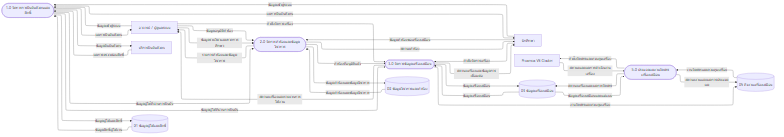
\includegraphics[width=1.0\textwidth]{Image/diagram/chapter3-dataflow-level0-vm-operations.png}
%     \caption{\fontSixTeen{แผนภาพการไหลของข้อมูลระดับ 0: กลุ่มกระบวนการจัดการคำร้องและเครื่องเสมือน}}
%     \label{fig3:data_flow_level_0_vm_operations}
% \end{figure}

% \begin{figure}[H]
%     \centering
%     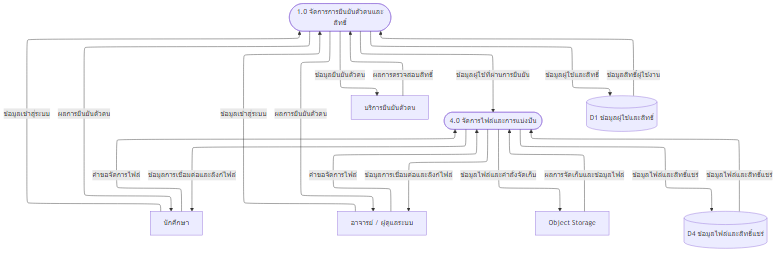
\includegraphics[width=1.0\textwidth]{Image/diagram/chapter3-dataflow-level0-storage.png}
%     \caption{\fontSixTeen{แผนภาพการไหลของข้อมูลระดับ 0: กลุ่มกระบวนการยืนยันตัวตนและจัดการไฟล์}}
%     \label{fig3:data_flow_level_0_storage}
% \end{figure}

\hspace*{1.3em} %ย่อหน้า
ในระดับแผนภาพการไหลของข้อมูลระดับที่ 1 (DFD Level 1) ตามภาพที่ \ref{fig3:data_flow_level_1_auth} – \ref{fig3:data_flow_level_1_vm} ได้ทำการขยายกระบวนการหลักจากระดับ 0 ให้เห็นรายละเอียดของกระแสข้อมูลภายในระบบมากขึ้น โดยยังคงรักษาหลัก \textit{Balancing} กล่าวคือ ข้อมูลเข้าและข้อมูลออกของแต่ละกระบวนการหลักต้องสอดคล้องกับสิ่งที่ปรากฏใน DFD ระดับ 0 และไม่สร้าง/ลบกระแสข้อมูลที่ไม่มีอยู่ในระดับก่อนหน้า ทั้งนี้สามารถสรุปแนวคิดสำคัญของกระบวนการระดับที่ 1 ได้ดังนี้

\begin{figure}[H]
    \centering
    % แผนภาพนี้ควรรีเจนจากไฟล์ Mermaid: docs/diagram/chapter3-dataflow-level1-process1.mmd
    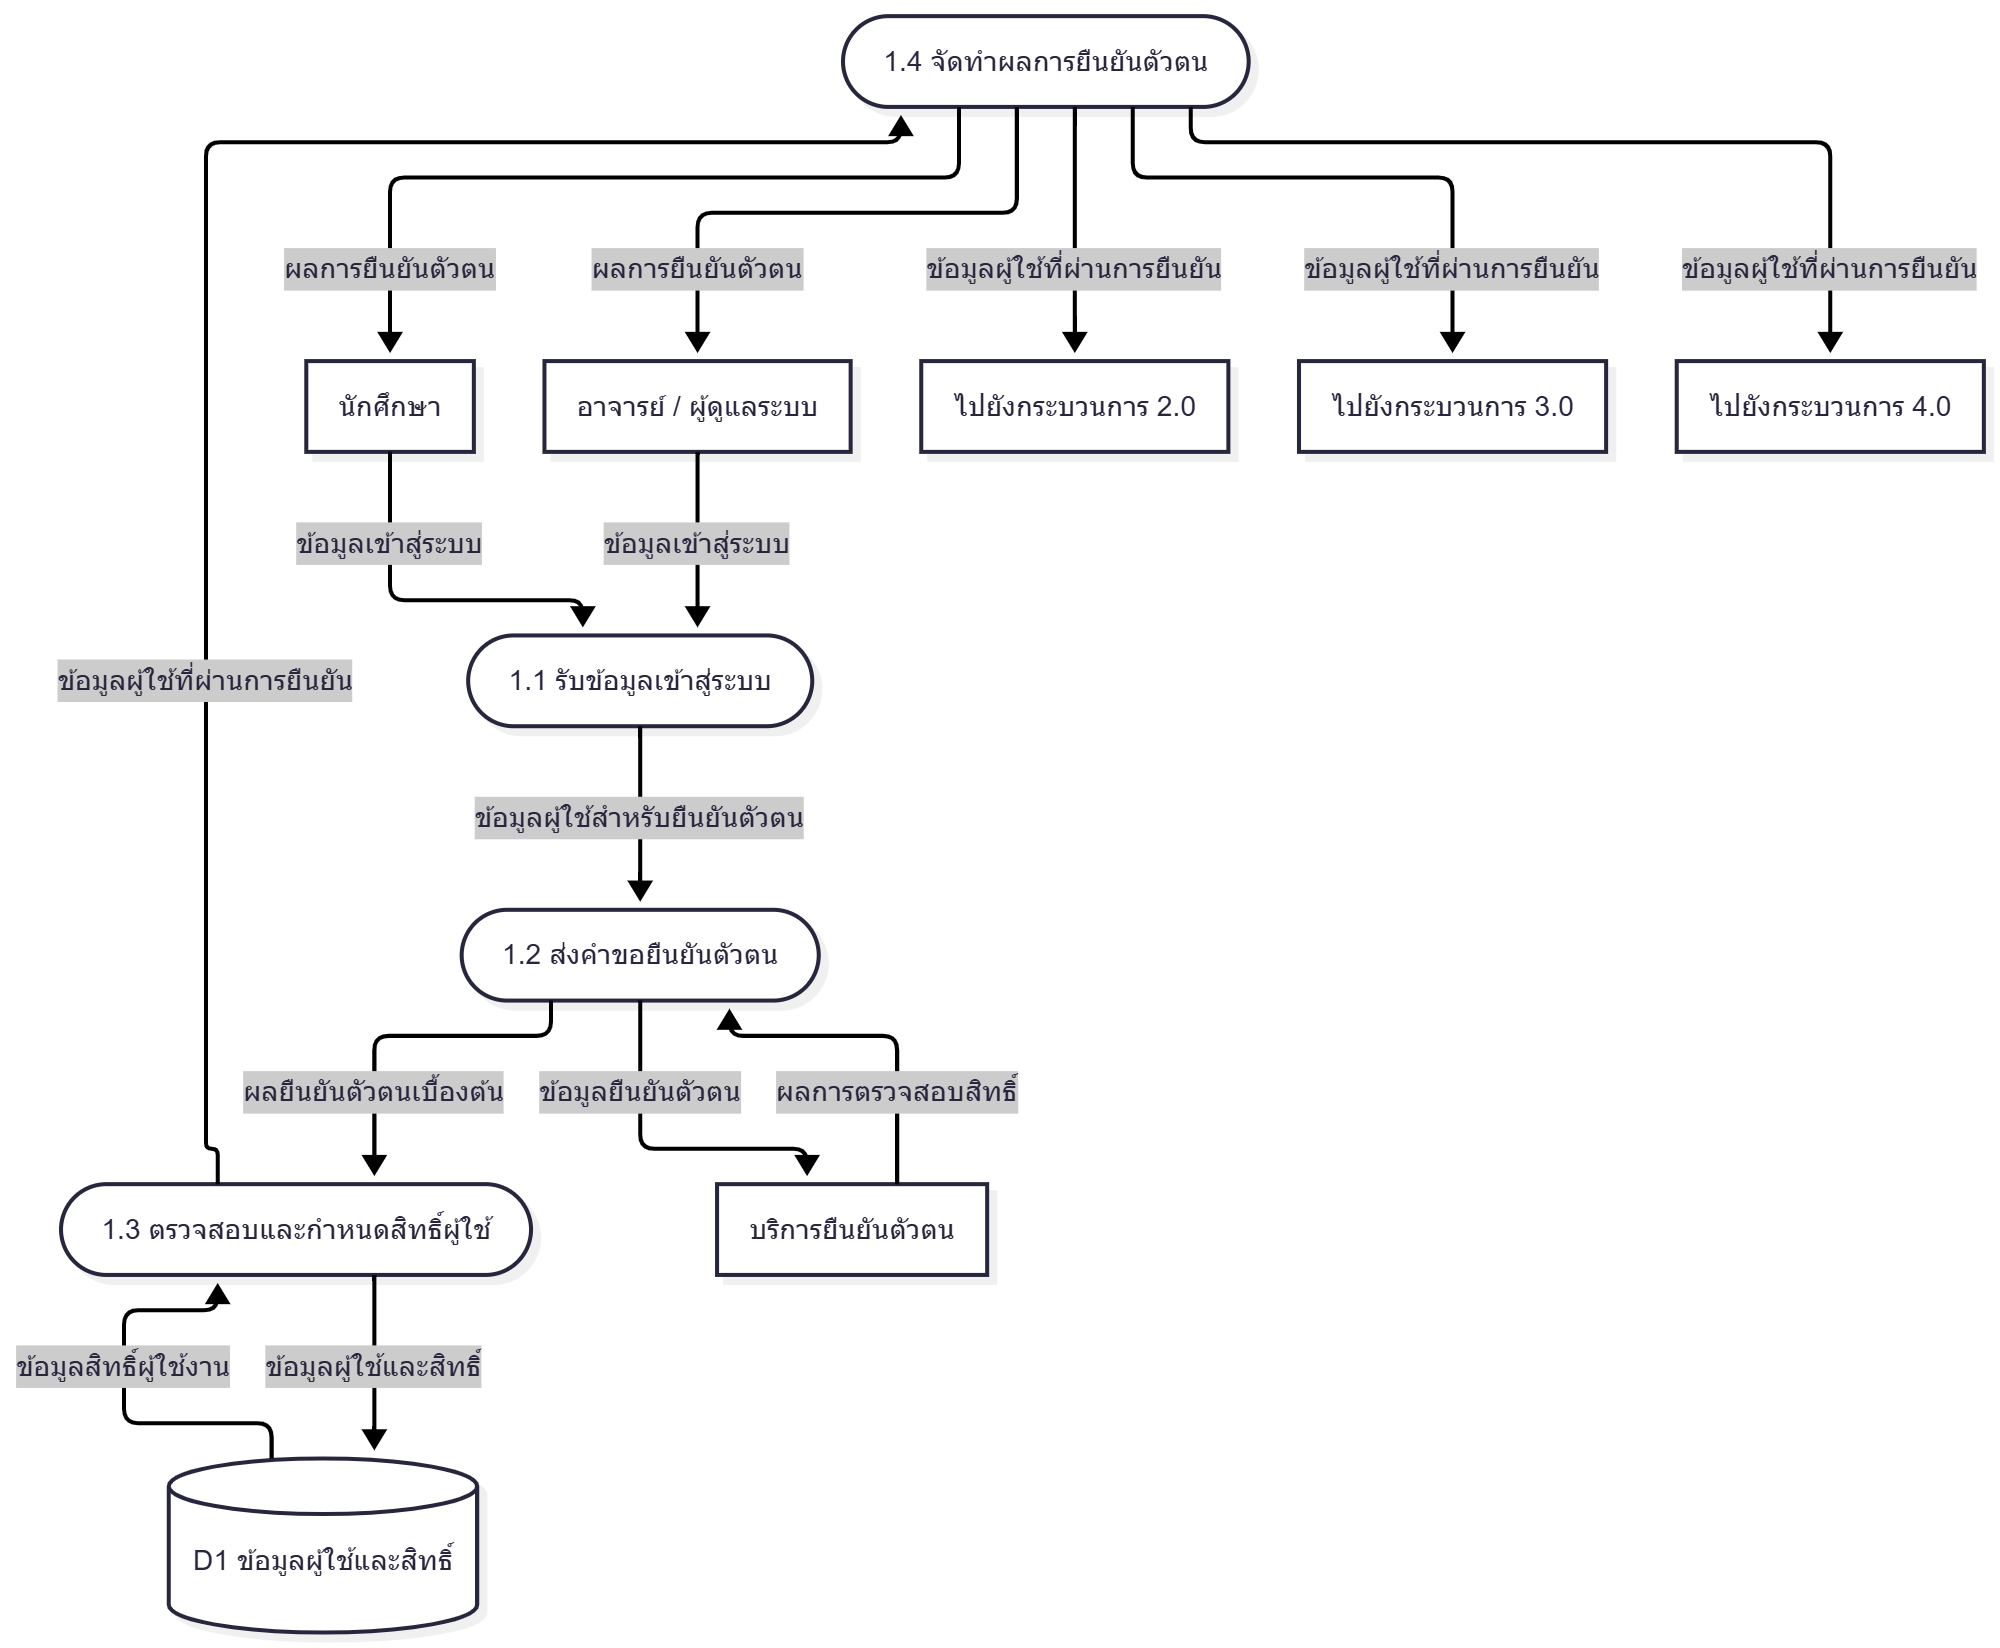
\includegraphics[width=1.0\textwidth]{Image/diagram/chapter3-dataflow-level1-process1.png}
    \caption{\fontSixTeen{แผนภาพการไหลของข้อมูลระดับที่ 1 ของกระบวนการ 1.0 การยืนยันตัวตนและกำหนดสิทธิ์ผู้ใช้}}
    \label{fig3:data_flow_level_1_auth}
\end{figure}

\hspace*{1.3em} %ย่อหน้า
\textbf{กระบวนการ 1.0 การยืนยันตัวตนและกำหนดสิทธิ์ผู้ใช้} (ภาพที่ \ref{fig3:data_flow_level_1_auth}) ทำหน้าที่เป็น \textit{gatekeeper} ของ API ทั้งระบบ โดยรับข้อมูลยืนยันตัวตนจากผู้ใช้ผ่าน Midori จากนั้นสร้าง/ตรวจสอบ Session และผูกกับข้อมูลผู้ใช้ในฐานข้อมูลเพื่อกำหนดบทบาท (ADMIN/INSTRUCTOR/STUDENT) เส้นทางนี้ให้บริการผ่านโมดูล better-auth ภายใน Momoi และใช้ฐานข้อมูลพร้อมกติกา RBAC ชุดเดียวกับบริการ API อื่น ๆ ผลลัพธ์คือ token/session ที่ใช้ซ้ำได้ในการเรียก API อื่น ๆ และข้อมูลสิทธิ์ที่ใช้ประกอบการอนุมัติการเข้าถึงทรัพยากร

\begin{figure}[H]
    \centering
    % แผนภาพนี้ควรรีเจนจากไฟล์ Mermaid: docs/diagram/chapter3-dataflow-level1-process2.mmd
    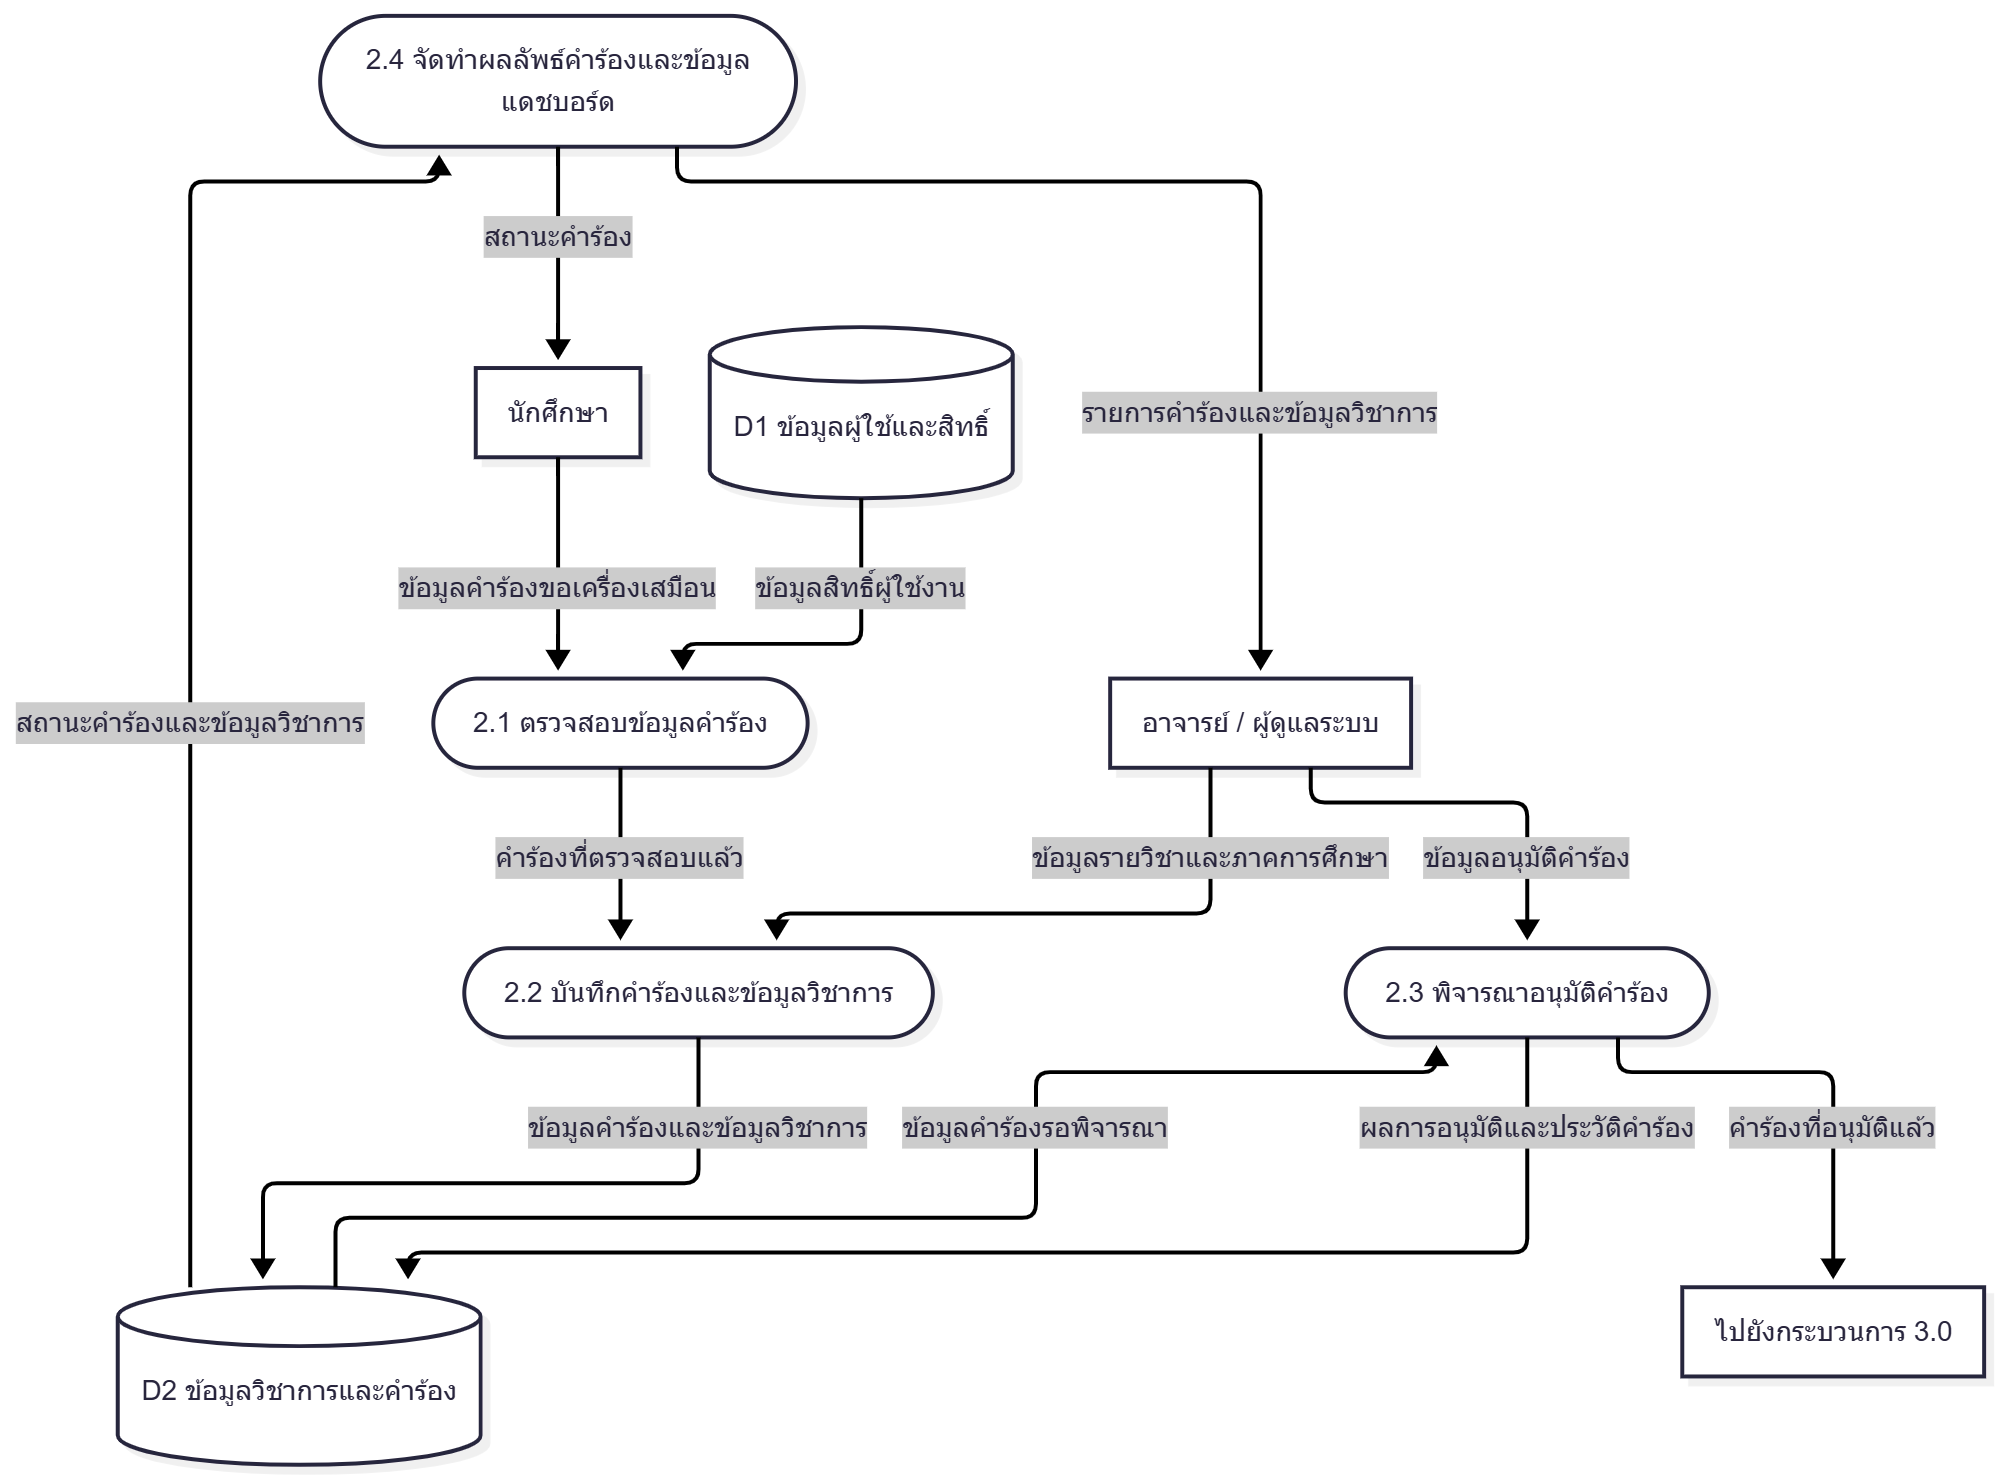
\includegraphics[width=1.0\textwidth]{Image/diagram/chapter3-dataflow-level1-process2.png}
    \caption{\fontSixTeen{แผนภาพการไหลของข้อมูลระดับที่ 1 ของกระบวนการ 2.0 การจัดการคำร้องและข้อมูลวิชาการ}}
    \label{fig3:data_flow_level_1_frontend}
\end{figure}

\hspace*{1.3em} %ย่อหน้า
\textbf{กระบวนการ 2.0 การจัดการคำร้องและข้อมูลวิชาการ} (ภาพที่ \ref{fig3:data_flow_level_1_frontend}) เน้นการจัดการข้อมูลเชิงโดเมนที่เกี่ยวข้องกับผู้ใช้และการเรียนการสอน เช่น รายวิชา/ภาคการศึกษา/ผู้สอน รวมถึงวงจรคำร้องขอเครื่องเสมือนและการตรวจสอบสิทธิ์ของผู้ยื่นคำร้อง จุดสำคัญคือข้อมูลคำร้องและประวัติการอนุมัติจะถูกจัดเก็บแบบเป็นโครงสร้างเพื่อให้สามารถตรวจสอบย้อนหลังได้ และสถานะคำร้องถูกส่งกลับไปยัง UI เพื่อสื่อสารความคืบหน้าให้ผู้ใช้

\begin{figure}[H]
    \centering
    % แผนภาพนี้ควรรีเจนจากไฟล์ Mermaid: docs/diagram/chapter3-dataflow-level1-process3.mmd
    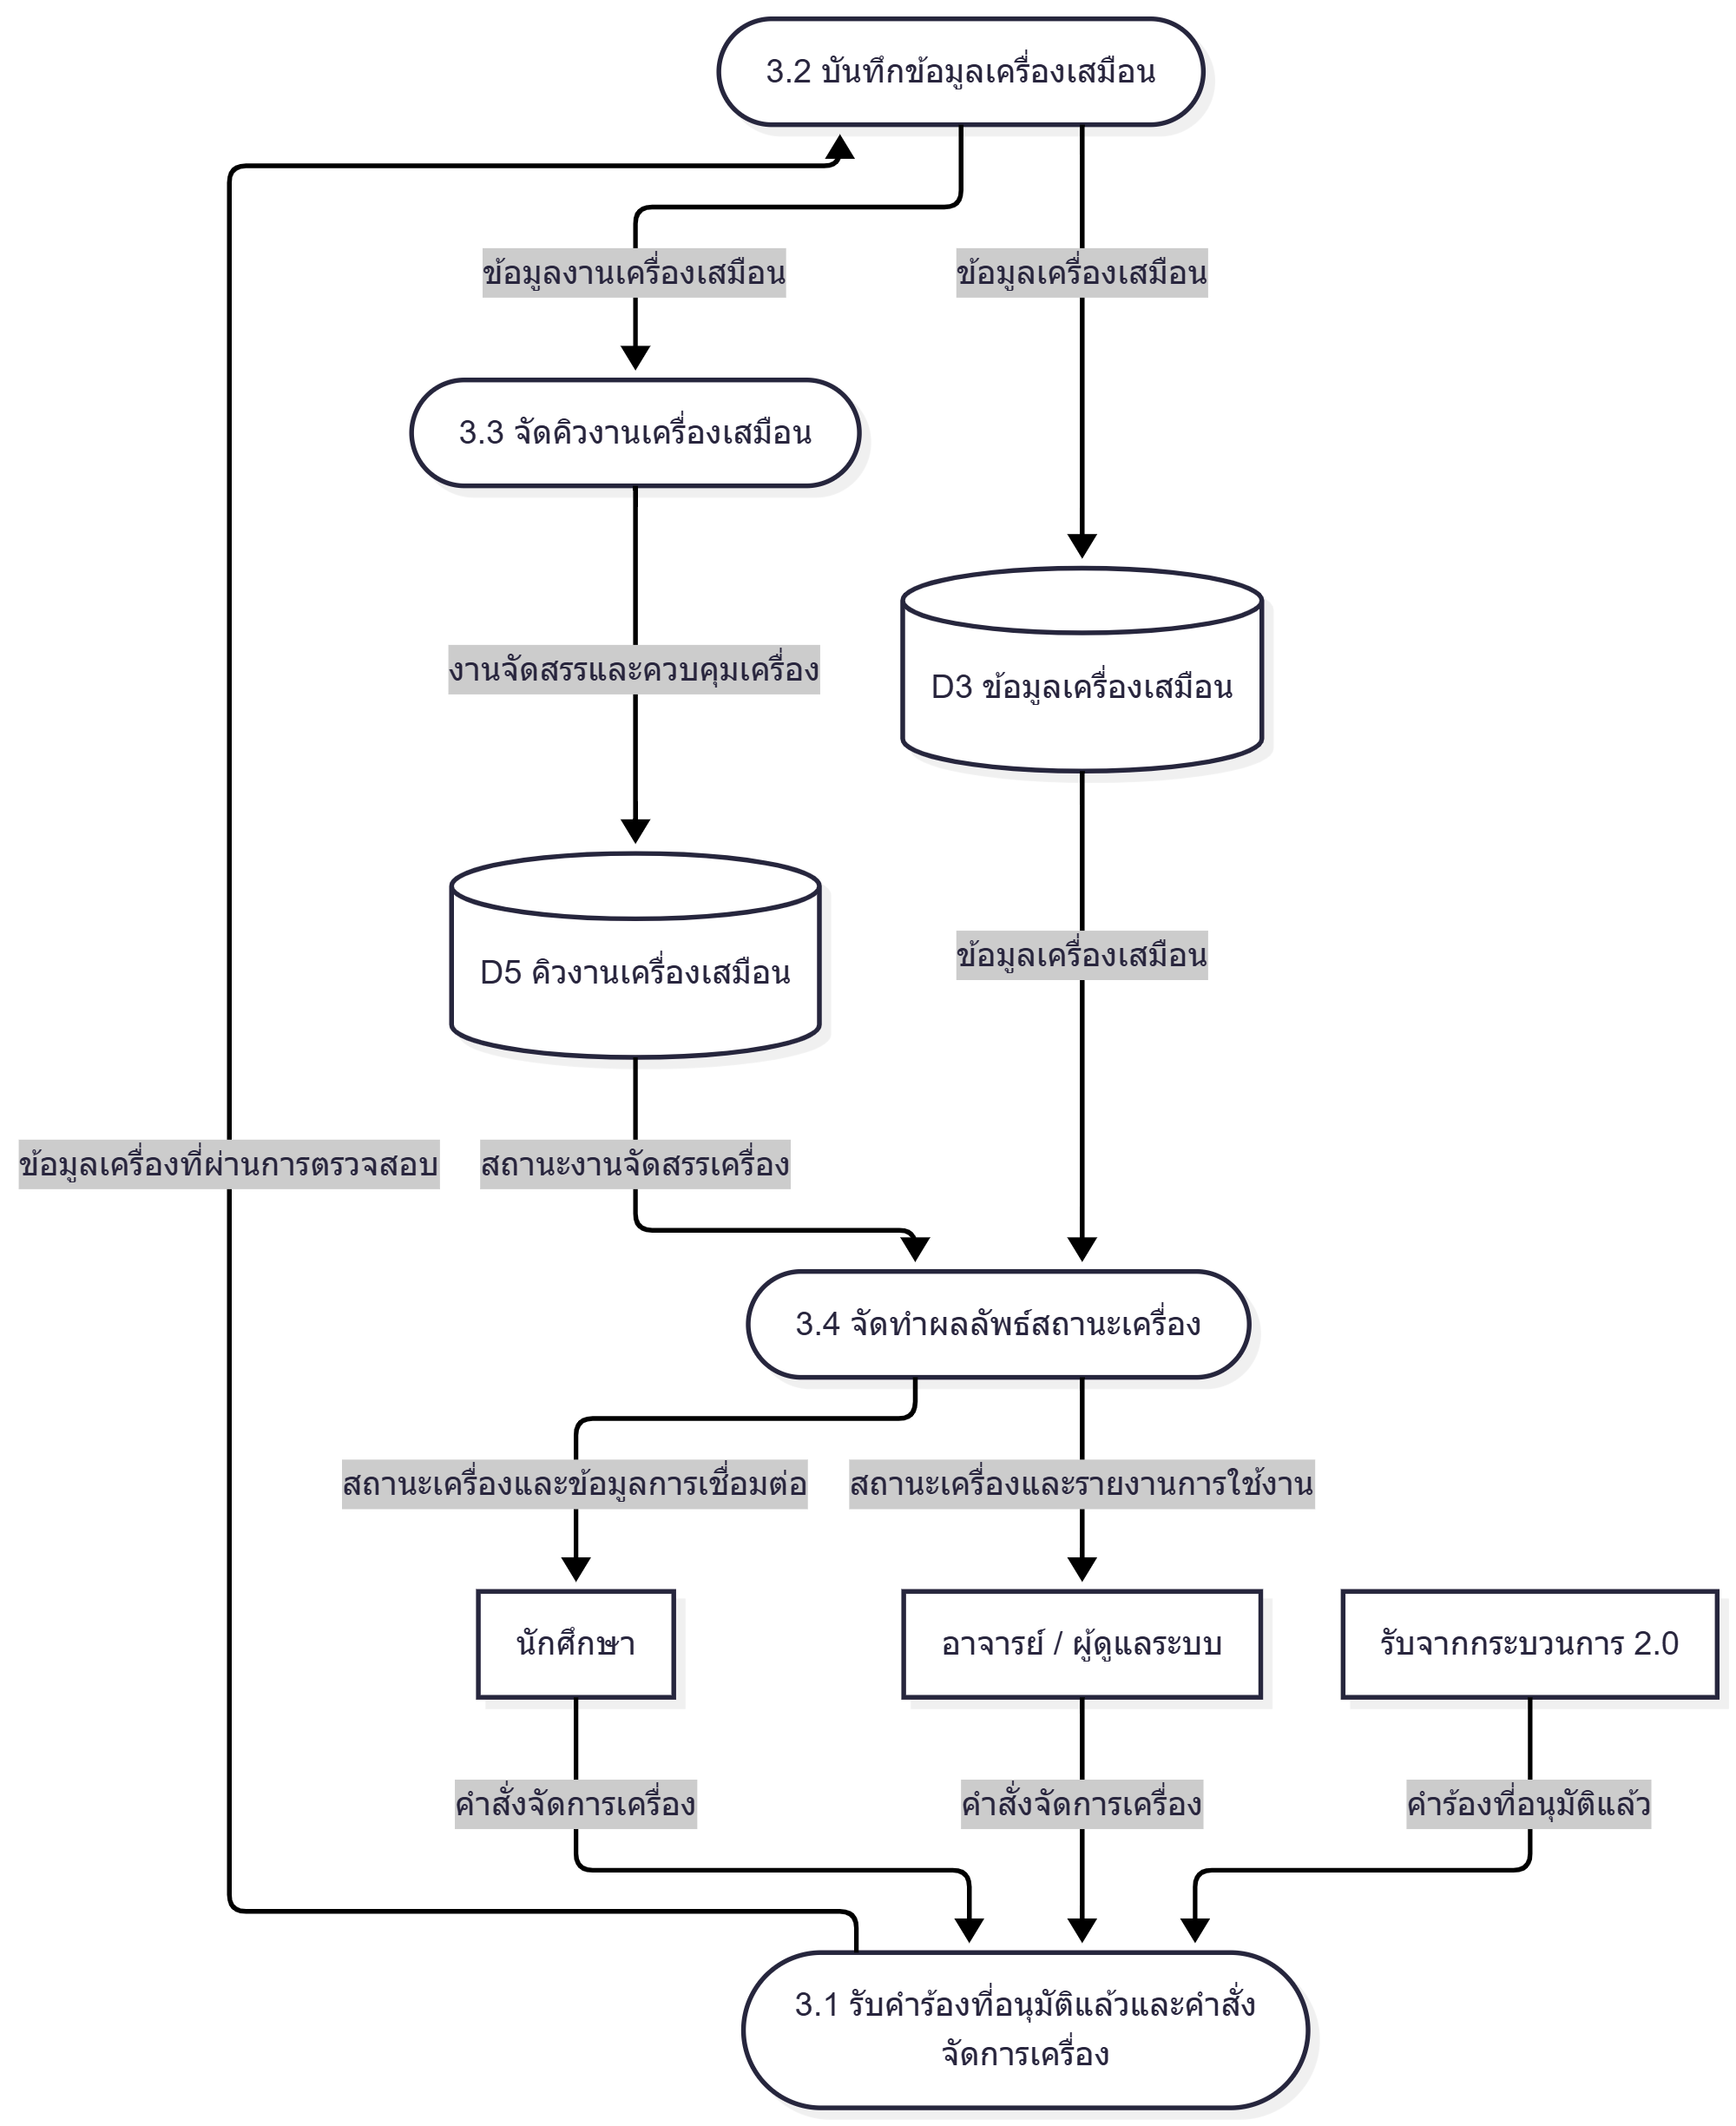
\includegraphics[width=0.95\textwidth]{Image/diagram/chapter3-dataflow-level1-process3.png}
    \caption{\fontSixTeen{แผนภาพการไหลของข้อมูลระดับที่ 1 ของกระบวนการ 3.0 การจัดการข้อมูลเครื่องเสมือน}}
    \label{fig3:data_flow_level_1_backend}
\end{figure}

\hspace*{1.3em} %ย่อหน้า
\textbf{กระบวนการ 3.0 การจัดการข้อมูลเครื่องเสมือน} (ภาพที่ \ref{fig3:data_flow_level_1_backend}) เป็นส่วนกลางของการจัดการ VM ในเชิงธุรกรรม โดยอ่าน/เขียนข้อมูล Instance และความสัมพันธ์กับทรัพยากร Proxmox VE ในฐานข้อมูล รวมถึงการตัดสินใจว่างานใดควรประมวลผลแบบทันที (เช่นการอ่านสถานะจากฐานข้อมูล) และงานใดควรส่งไปประมวลผลแบบอะซิงโครนัสผ่านคิว (เช่นการสร้าง/ลบ/สั่งเริ่ม-หยุด VM) เพื่อให้ API ตอบสนองรวดเร็วและรองรับการ retry ได้อย่างปลอดภัย

\begin{figure}[H]
    \centering
    % แผนภาพนี้ควรรีเจนจากไฟล์ Mermaid: docs/diagram/chapter3-dataflow-level1-process4.mmd
    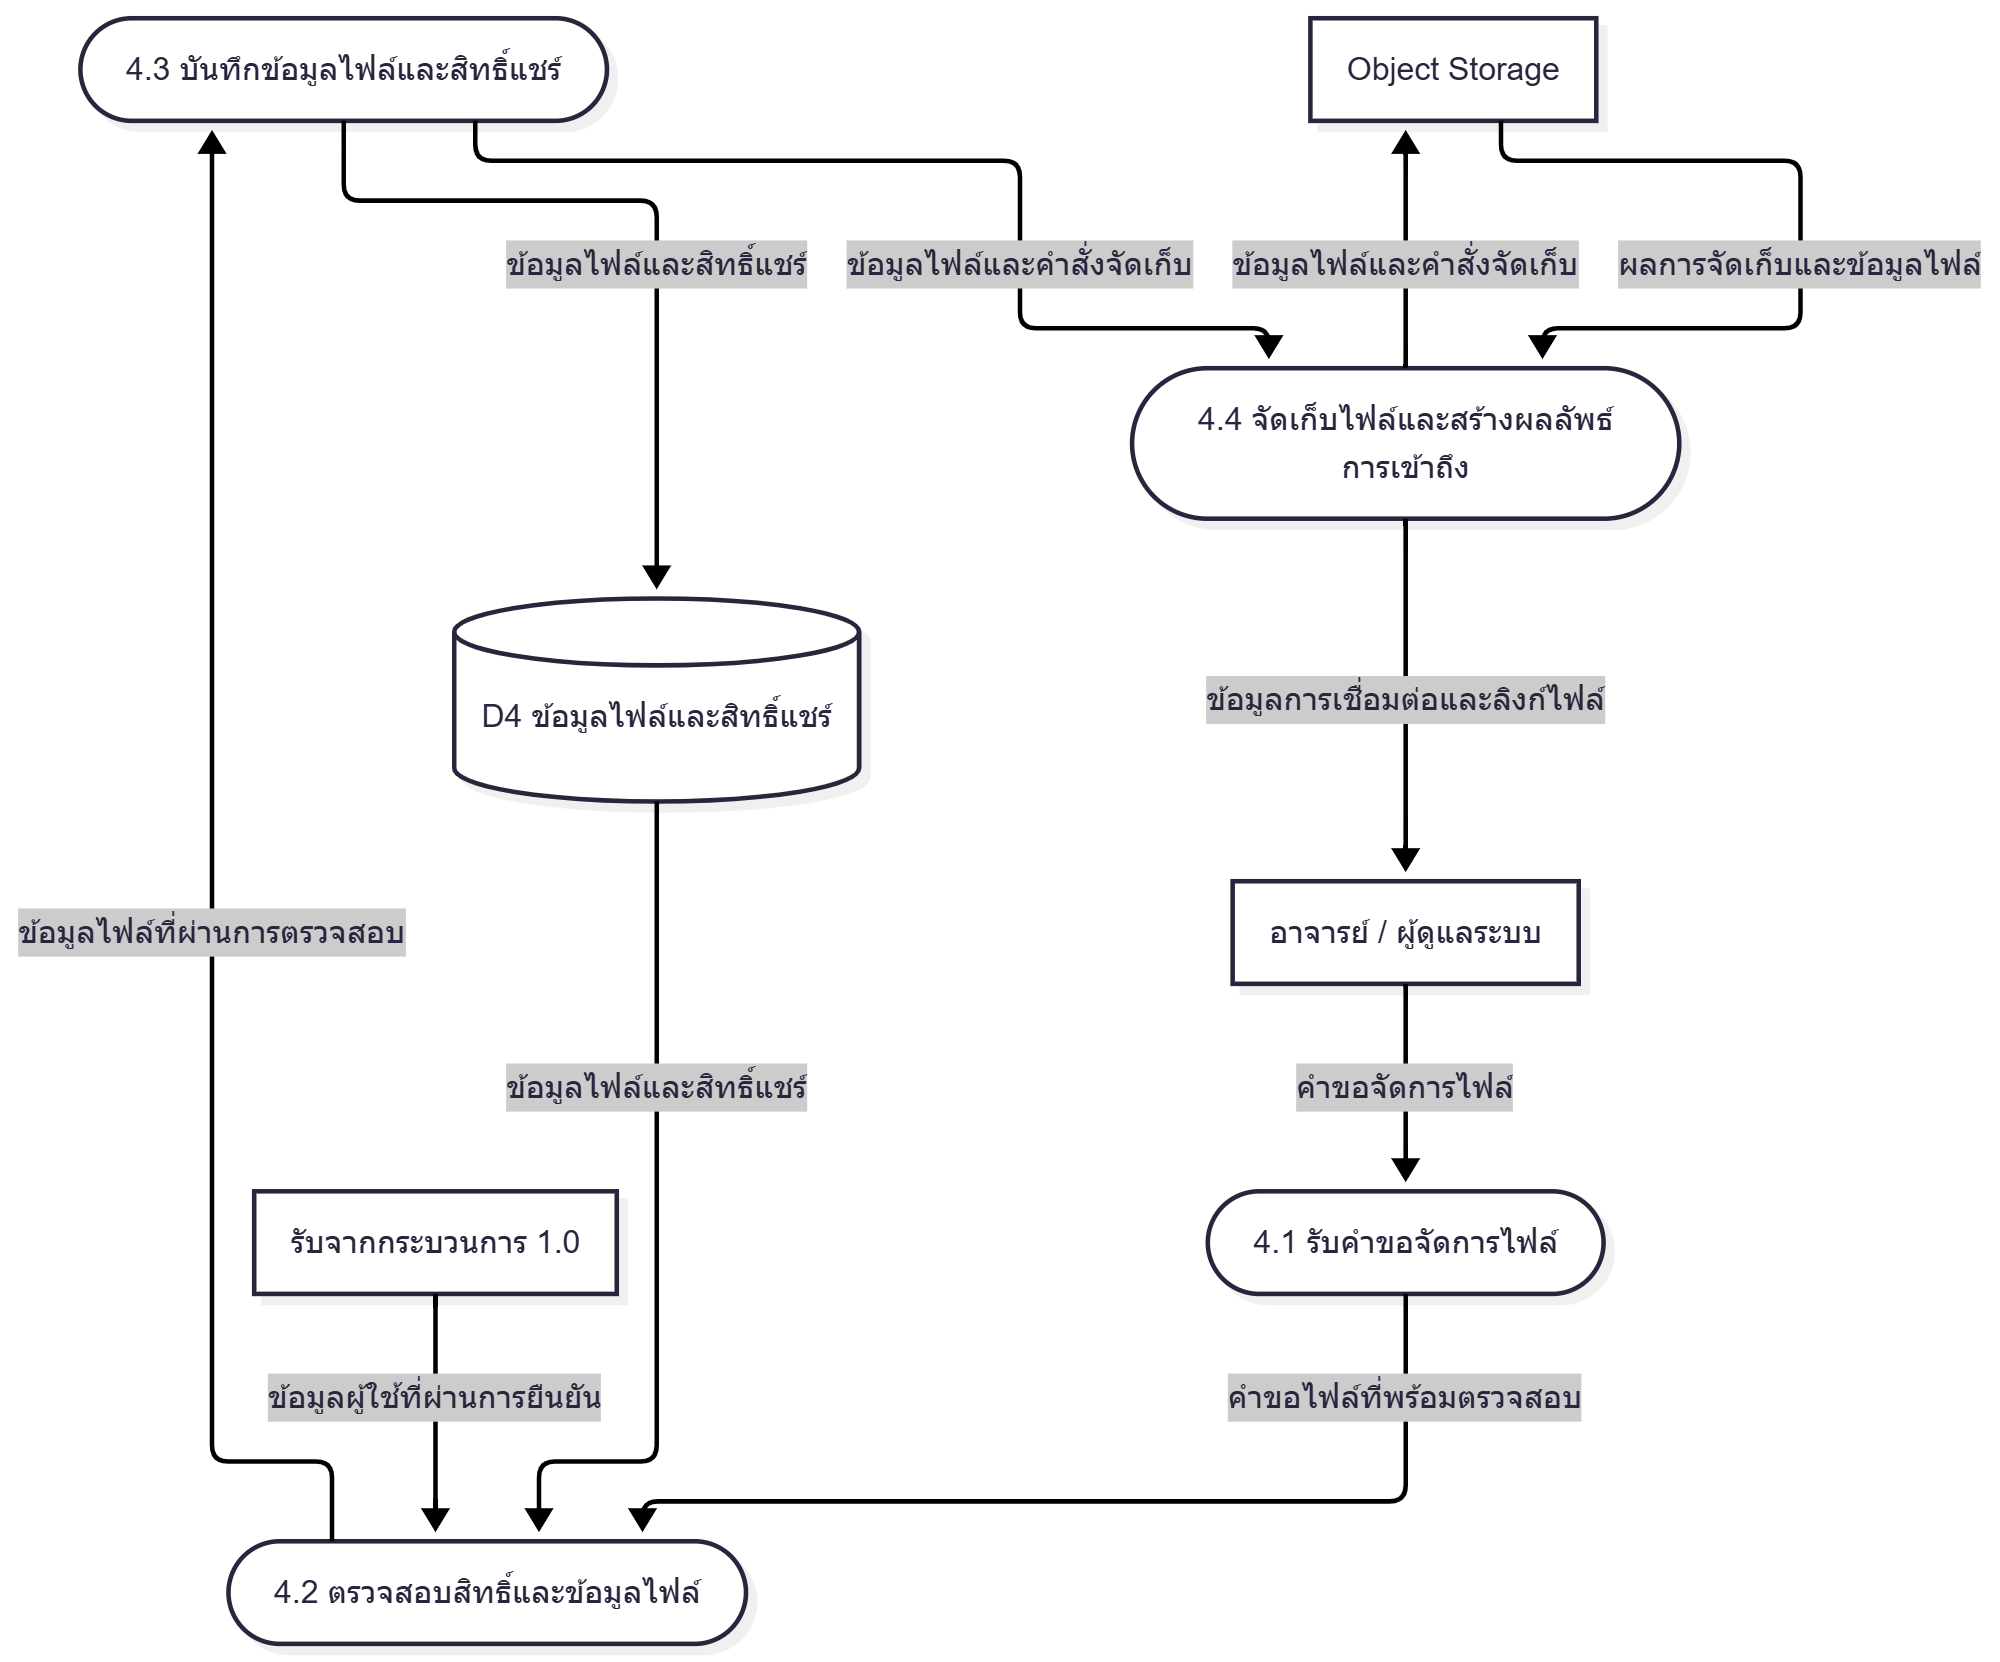
\includegraphics[width=1.0\textwidth]{Image/diagram/chapter3-dataflow-level1-process4.png}
    \caption{\fontSixTeen{แผนภาพการไหลของข้อมูลระดับที่ 1 ของกระบวนการ 4.0 การจัดการไฟล์และสิทธิ์การเข้าถึง}}
    \label{fig3:data_flow_level_1_storage}
\end{figure}

\hspace*{1.3em} %ย่อหน้า
\textbf{กระบวนการ 4.0 การจัดการไฟล์และสิทธิ์การเข้าถึง} (ภาพที่ \ref{fig3:data_flow_level_1_storage}) แยกการจัดการ \textit{เมทาดาทา} (เช่นชื่อไฟล์, owner, permission, เวลาอัปโหลด) ออกจาก \textit{ข้อมูลไฟล์จริง} ที่อยู่ใน Object Storage โดยกระบวนการนี้จึงต้องจัดการทั้งสิทธิ์เข้าถึงและการออกลิงก์/โทเคนการเข้าถึงตามนโยบายของระบบ เพื่อให้การควบคุมสิทธิ์สอดคล้องกับบทบาทผู้ใช้และบริบทของรายวิชา/คำร้อง

\begin{figure}[H]
    \centering
    % แผนภาพนี้ควรรีเจนจากไฟล์ Mermaid: docs/diagram/chapter3-dataflow-level1-process5.mmd
    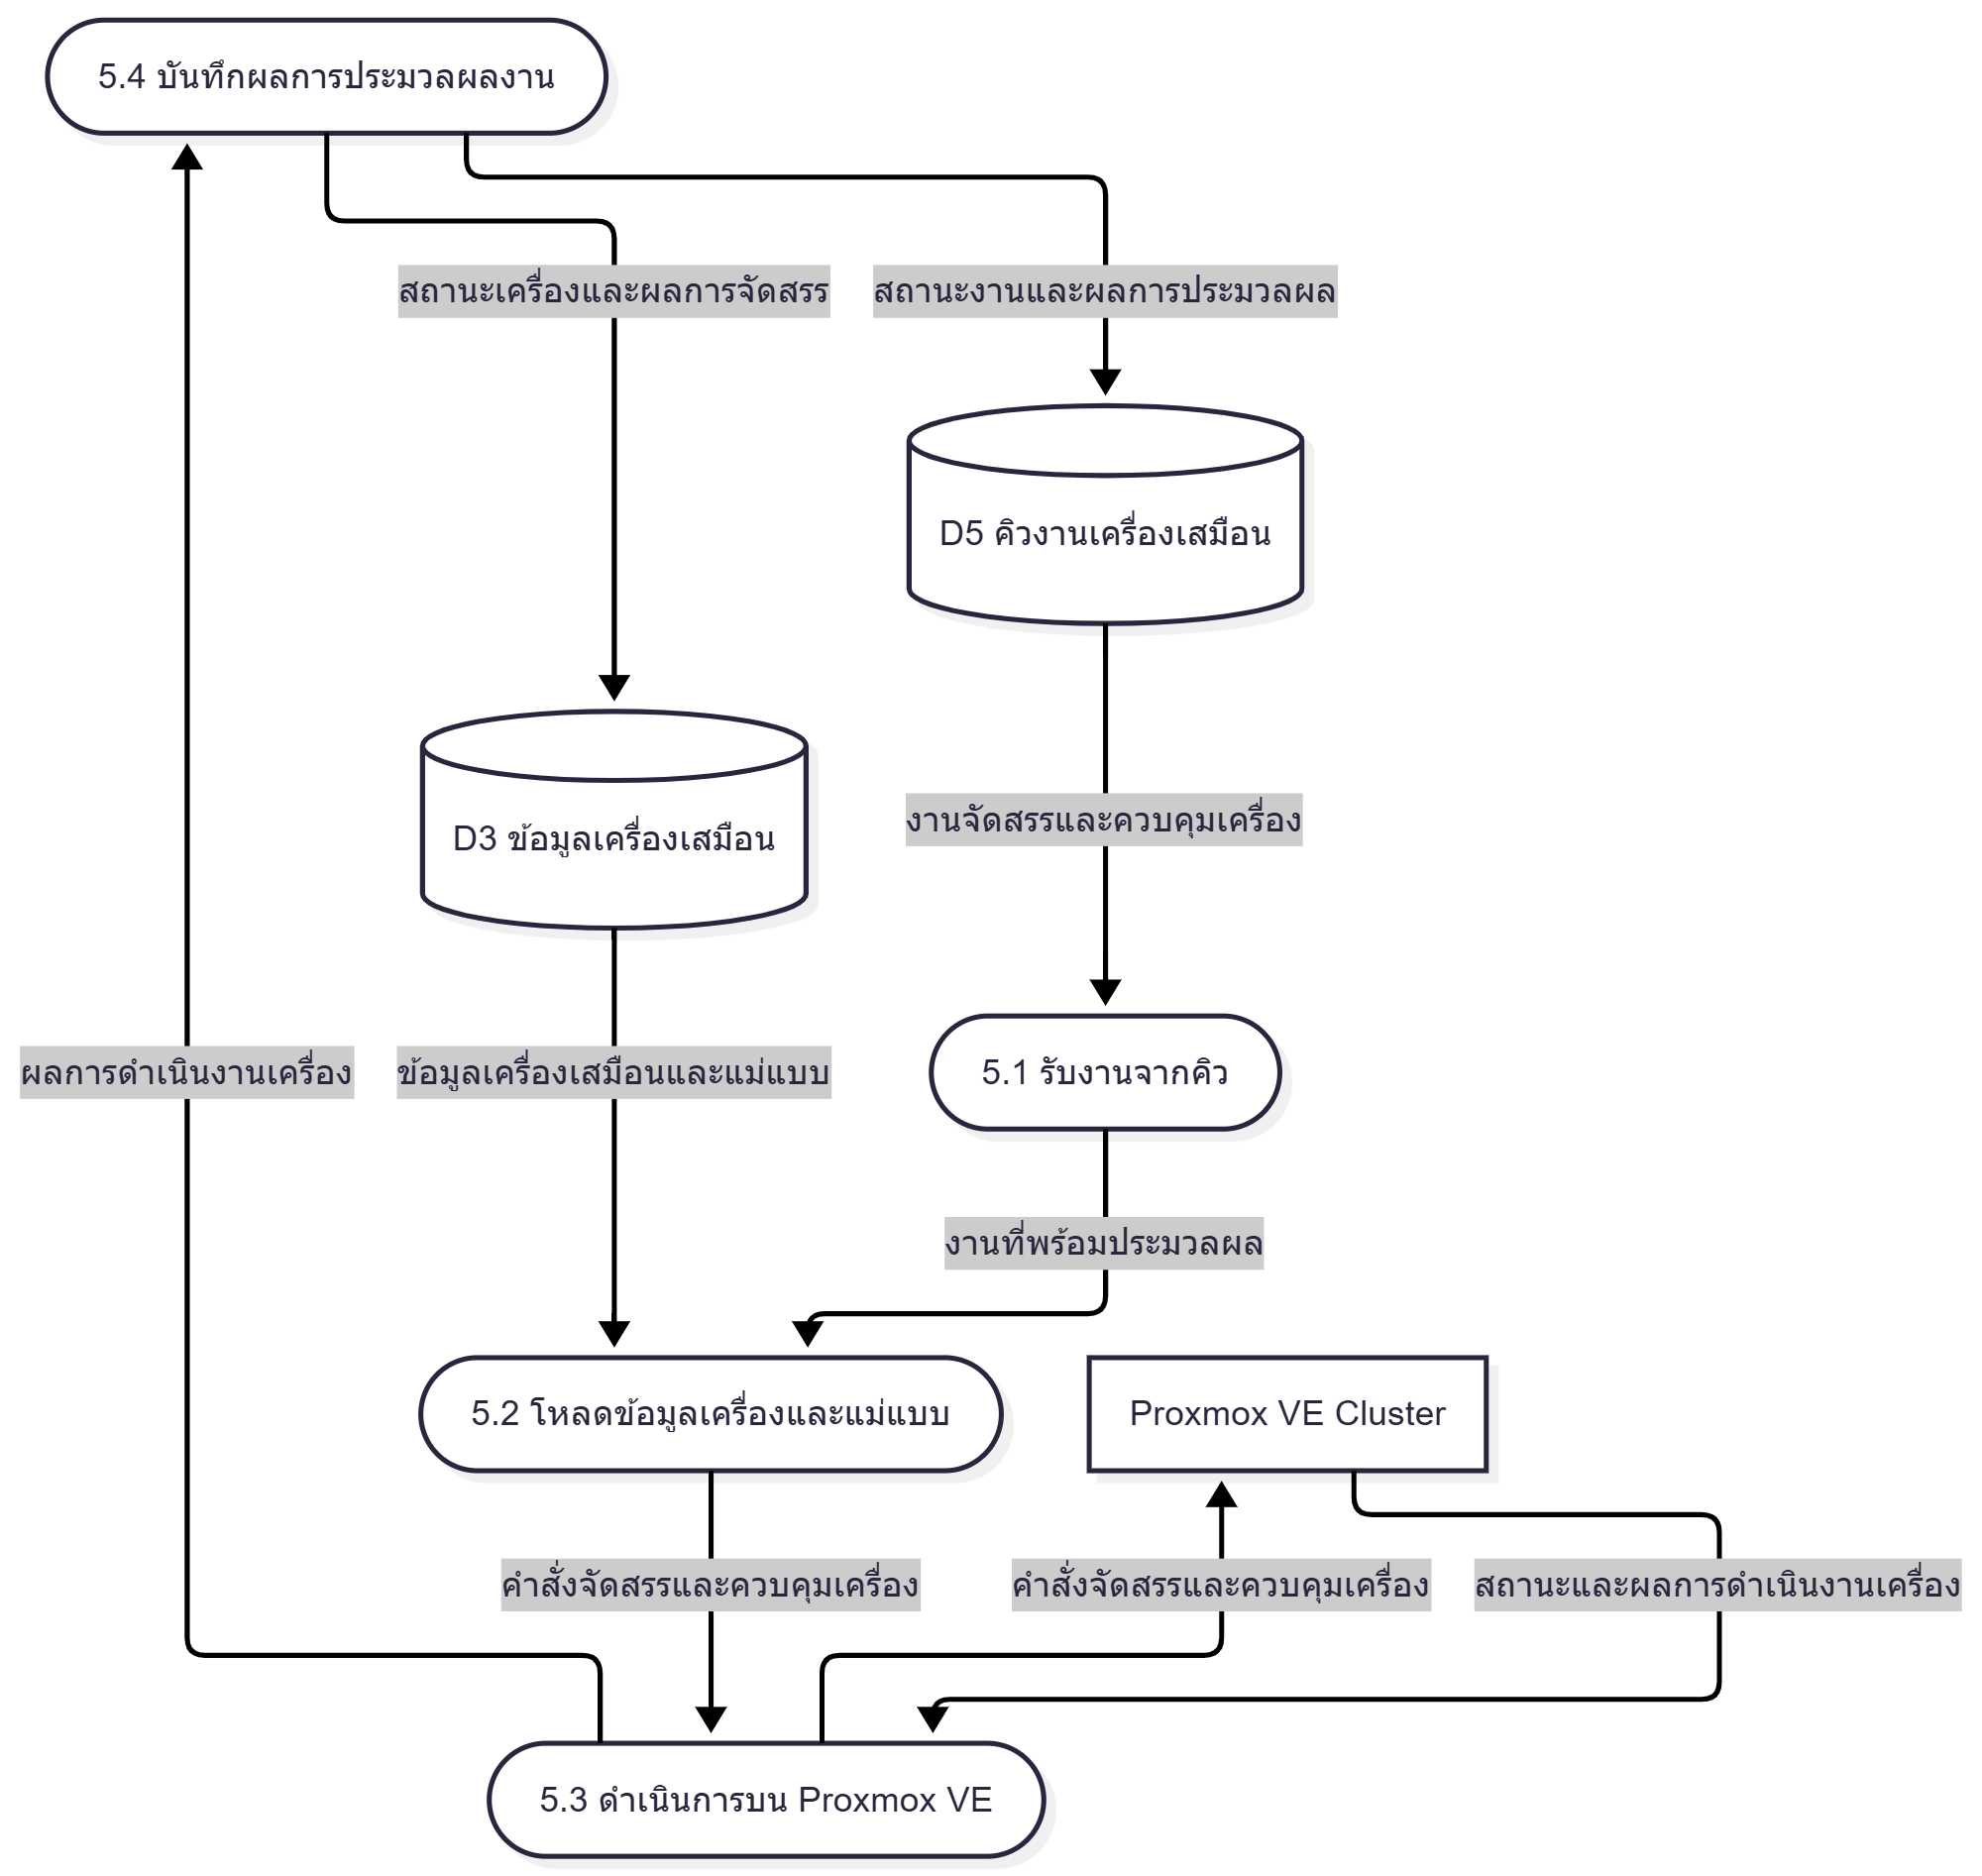
\includegraphics[width=1.0\textwidth]{Image/diagram/chapter3-dataflow-level1-process5.png}
    \caption{\fontSixTeen{แผนภาพการไหลของข้อมูลระดับที่ 1 ของกระบวนการ 5.0 การประมวลผลงานจัดสรรเครื่องเสมือน}}
    \label{fig3:data_flow_level_1_vm}
\end{figure}

\hspace*{1.3em} %ย่อหน้า
\textbf{กระบวนการ 5.0 การประมวลผลงานจัดสรรเครื่องเสมือน} (ภาพที่ \ref{fig3:data_flow_level_1_vm}) แสดงบทบาทของ worker (Yuzu) ในการรับงานจากคิวและเรียก Proxmox VE จริง โดยผลลัพธ์ที่ได้จาก Proxmox VE (สำเร็จ/ล้มเหลว/สถานะระหว่างทาง) จะถูกนำกลับมาอัปเดตฐานข้อมูล เพื่อให้ Midori และ Momoi แสดงสถานะล่าสุดแก่ผู้ใช้ได้จากแหล่งข้อมูลเดียวกัน (single source of truth)

\hspace*{1.3em} %ย่อหน้า
สำหรับการวิเคราะห์เชิงลึกเพิ่มเติม ได้จัดทำแผนภาพการไหลของข้อมูลระดับที่ 2 เพื่อขยายกระบวนการย่อยที่มีความซับซ้อน ได้แก่ การพิจารณาอนุมัติคำร้องในกระบวนการ 2.3 การรับคำร้องที่อนุมัติแล้วและจัดเตรียมงานในกระบวนการ 3.1 การส่งงานเข้าคิวในกระบวนการ 3.3 และการดำเนินการบน Proxmox VE ในกระบวนการ 5.3 ทั้งนี้การกำหนดชื่อกระแสข้อมูลในแต่ละระดับถูกจัดให้สอดคล้องกันตามหลัก Balancing ของ DFD ดังแสดงในภาพที่ \ref{fig3:data_flow_level_2_approval} – \ref{fig3:data_flow_level_2_pve}

\hspace*{1.3em} %ย่อหน้า
ในระดับ DFD Level 2 การขยายรายละเอียดมีเป้าหมายเพื่อทำให้เห็น \textbf{จุดตัดสินใจ (decision points)} และ \textbf{จุดที่ต้องรักษาความถูกต้องของข้อมูล (consistency points)} ของระบบอย่างชัดเจน โดยเฉพาะกระบวนการที่เกี่ยวข้องกับการอนุมัติ (ต้องตรวจสอบสิทธิ์และบันทึกประวัติ) และกระบวนการที่เกี่ยวข้องกับงานระยะยาว (ต้องส่งเข้าคิวและรองรับการ retry) ซึ่งสามารถอธิบายกลไกสำคัญได้ดังนี้

\begin{figure}[H]
    \centering
    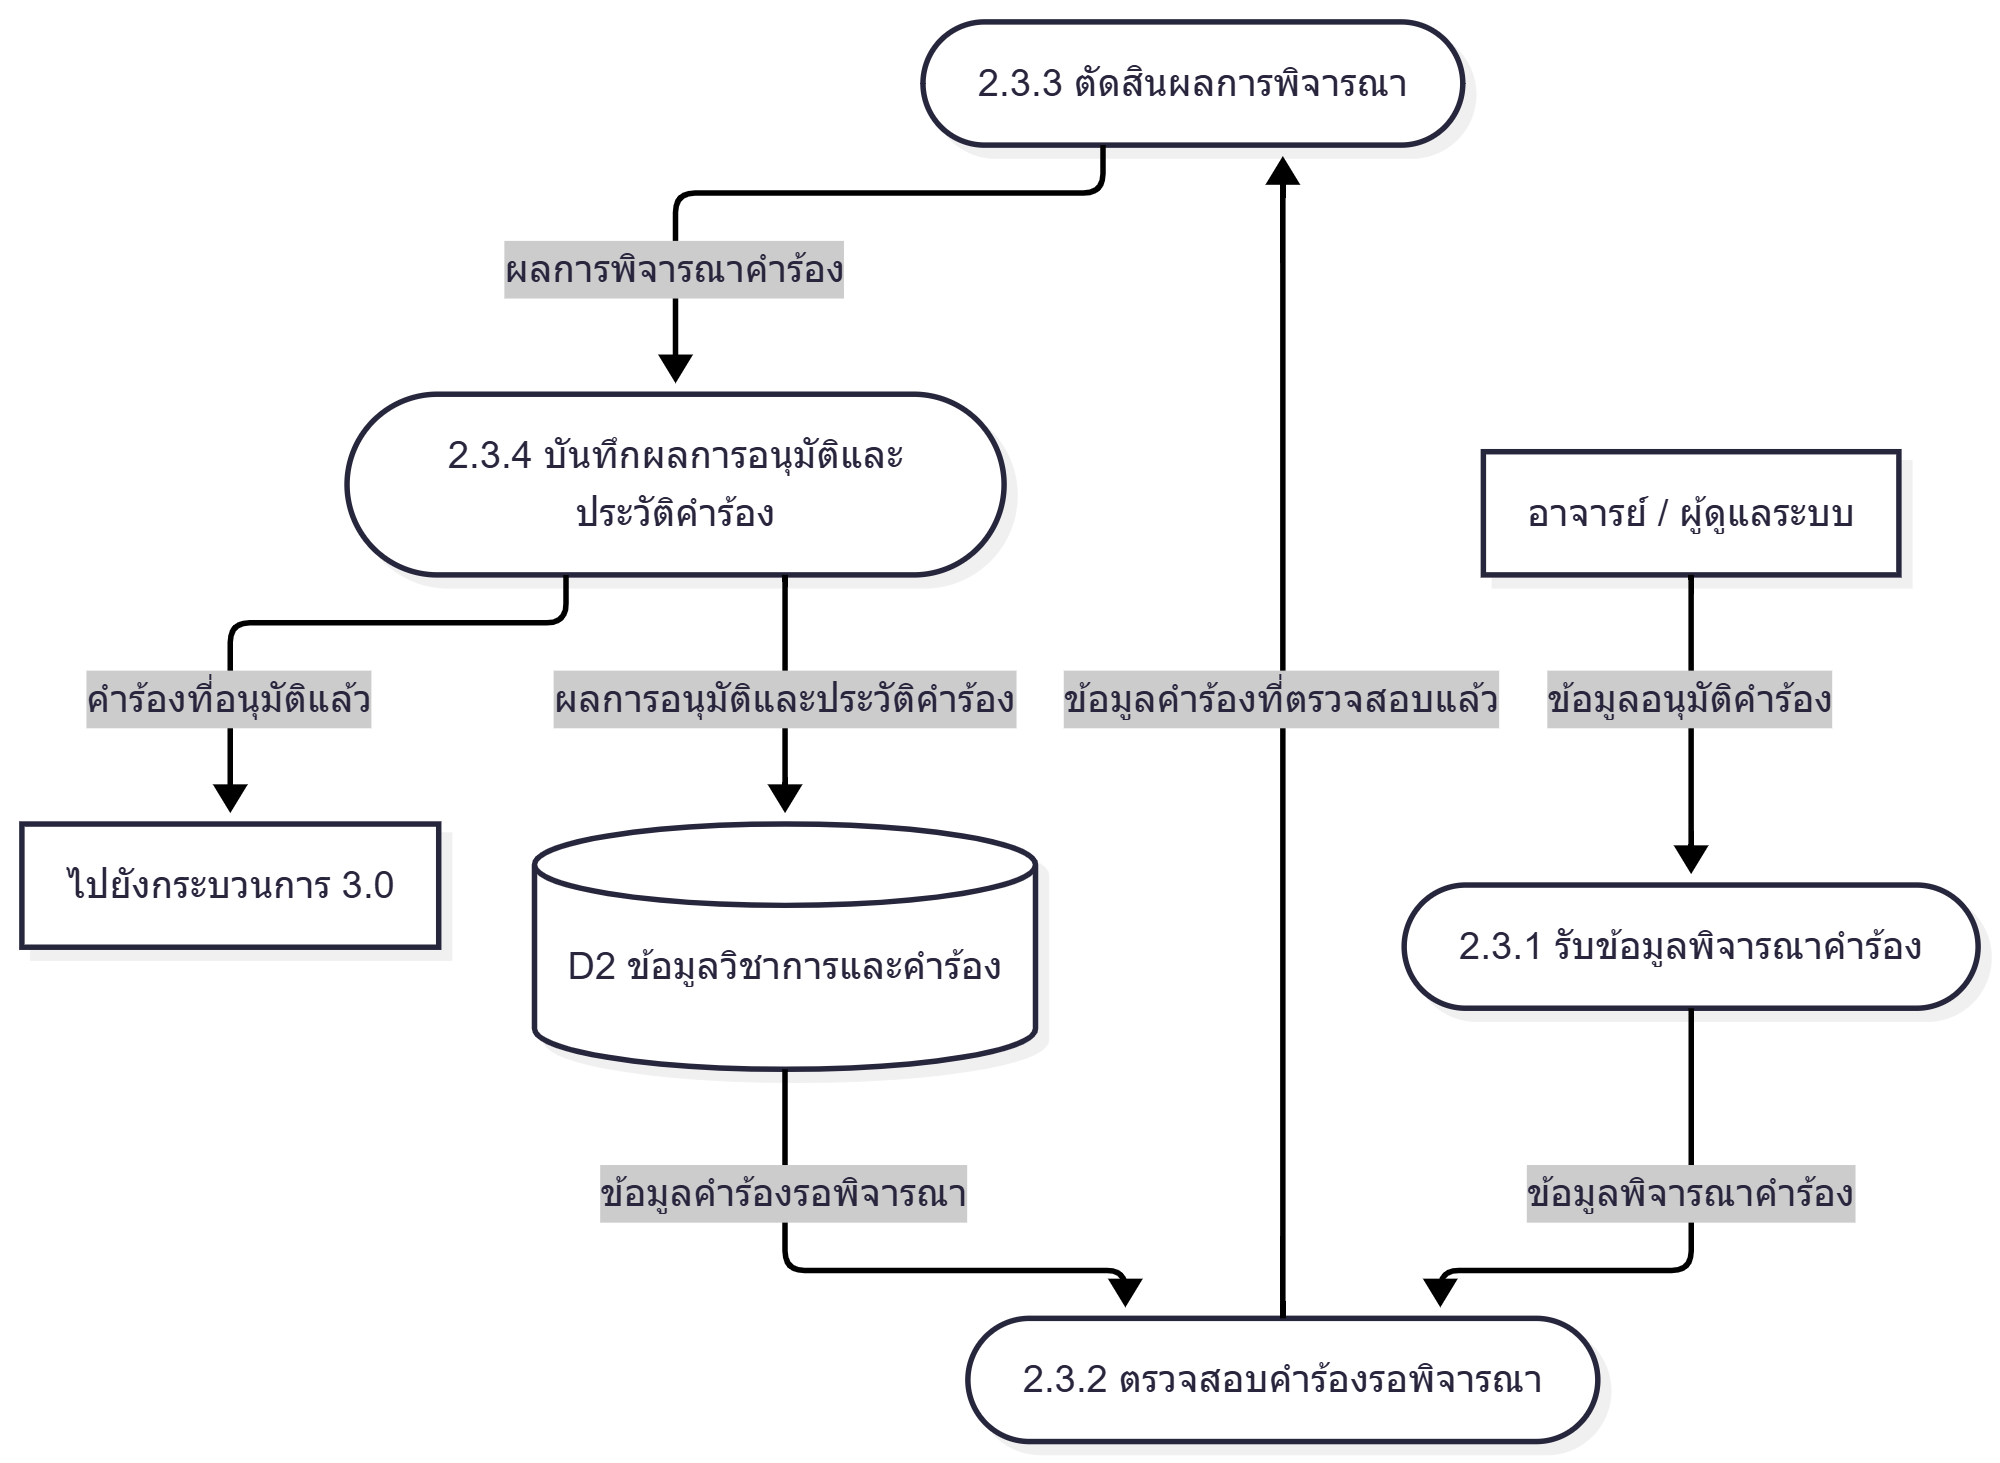
\includegraphics[width=1.0\textwidth]{Image/diagram/chapter3-dataflow-level2-process2-3.png}
    \caption{\fontSixTeen{แผนภาพการไหลของข้อมูลระดับที่ 2 ของกระบวนการ 2.3 การพิจารณาอนุมัติคำร้อง}}
    \label{fig3:data_flow_level_2_approval}
\end{figure}

\hspace*{1.3em} %ย่อหน้า
\textbf{กระบวนการ 2.3 การพิจารณาอนุมัติคำร้อง} (ภาพที่ \ref{fig3:data_flow_level_2_approval}) เริ่มจากผู้ดูแลระบบ/อาจารย์ส่งคำสั่งอนุมัติหรือปฏิเสธคำร้อง ระบบจะตรวจสอบสิทธิ์ของผู้ดำเนินการและสถานะคำร้องปัจจุบันก่อน (เพื่อป้องกันการอนุมัติซ้ำหรืออนุมัติคำร้องที่ถูกยกเลิกแล้ว) จากนั้นจึงอัปเดตสถานะคำร้องในฐานข้อมูล พร้อมบันทึกประวัติการตัดสินใจลงในตาราง audit log เพื่อใช้ตรวจสอบย้อนหลัง และส่งผลลัพธ์/สถานะใหม่กลับไปยัง UI

\begin{figure}[H]
    \centering
    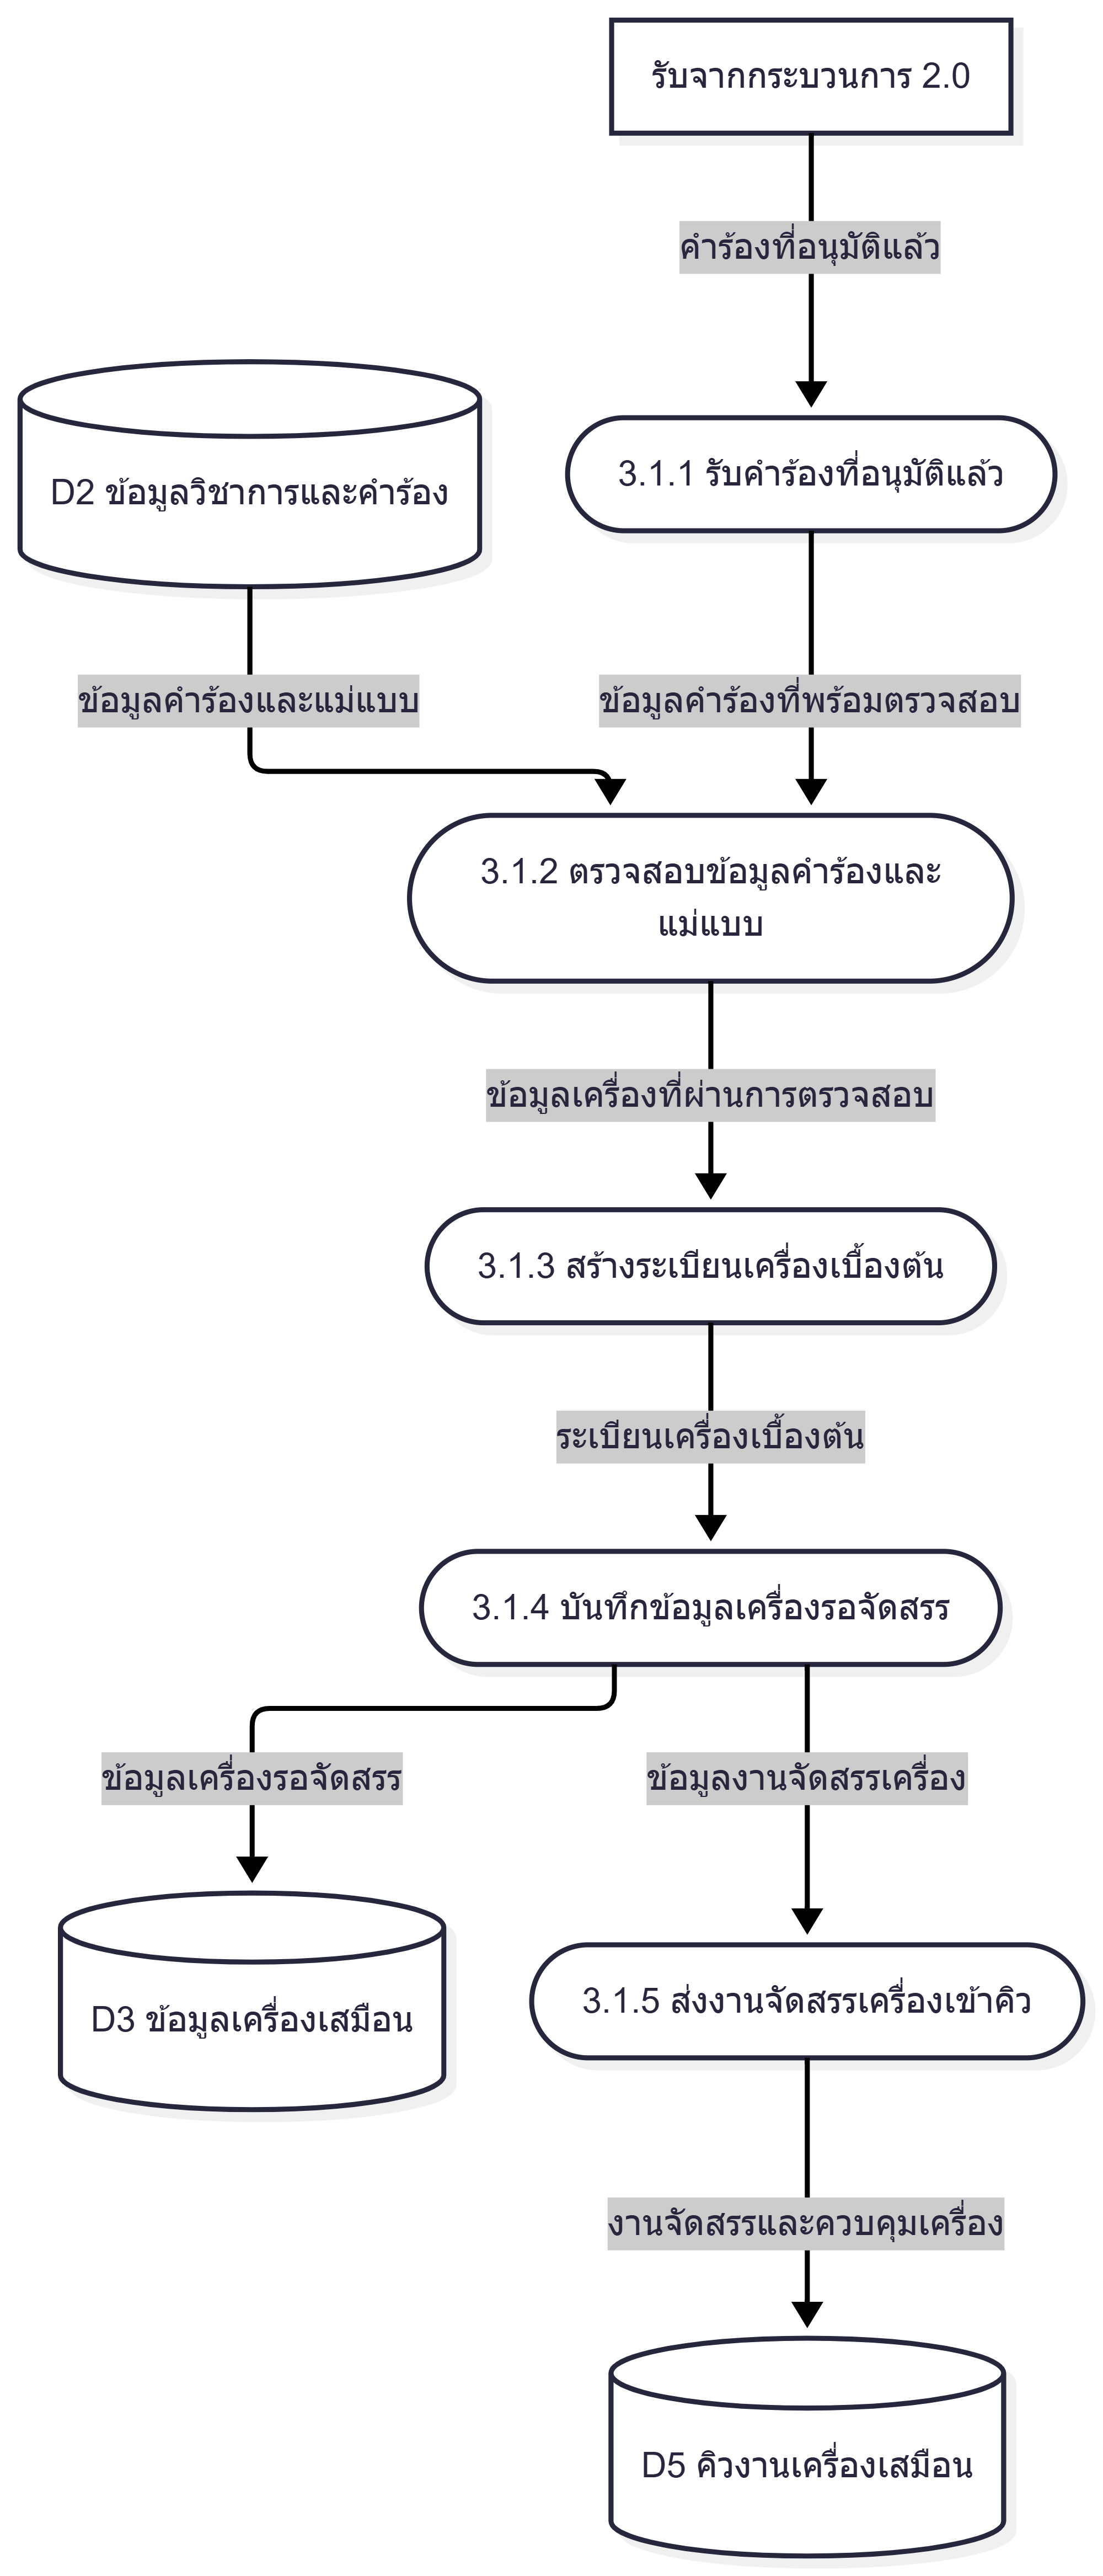
\includegraphics[width=0.50\textwidth]{Image/diagram/chapter3-dataflow-level2-process3-1.png}
    \caption{\fontSixTeen{แผนภาพการไหลของข้อมูลระดับที่ 2 ของกระบวนการ 3.1 การรับคำร้องที่อนุมัติแล้วและจัดเตรียมงาน}}
    \label{fig3:data_flow_level_2_provision}
\end{figure}

\hspace*{1.3em} %ย่อหน้า
\textbf{กระบวนการ 3.1 การรับคำร้องที่อนุมัติแล้วและจัดเตรียมงาน} (ภาพที่ \ref{fig3:data_flow_level_2_provision}) เมื่อคำร้องถูกอนุมัติ ระบบจะดึงข้อมูลที่จำเป็นจากฐานข้อมูล (เช่น รายละเอียดผู้ใช้ รายวิชา เทมเพลต VM โหนด/เครือข่ายที่เกี่ยวข้อง) เพื่อจัดเตรียม \textit{แผนการดำเนินงาน} (provision plan) และสร้างระเบียน Instance/งานที่เกี่ยวข้องในสถานะเริ่มต้น จุดนี้มักเน้นความสอดคล้องของข้อมูล เช่น ต้องผูกคำร้องกับ instanceId ที่ชัดเจน และกำหนดสถานะเพื่อรองรับการติดตามความคืบหน้าในขั้นถัดไป

\begin{figure}[H]
    \centering
    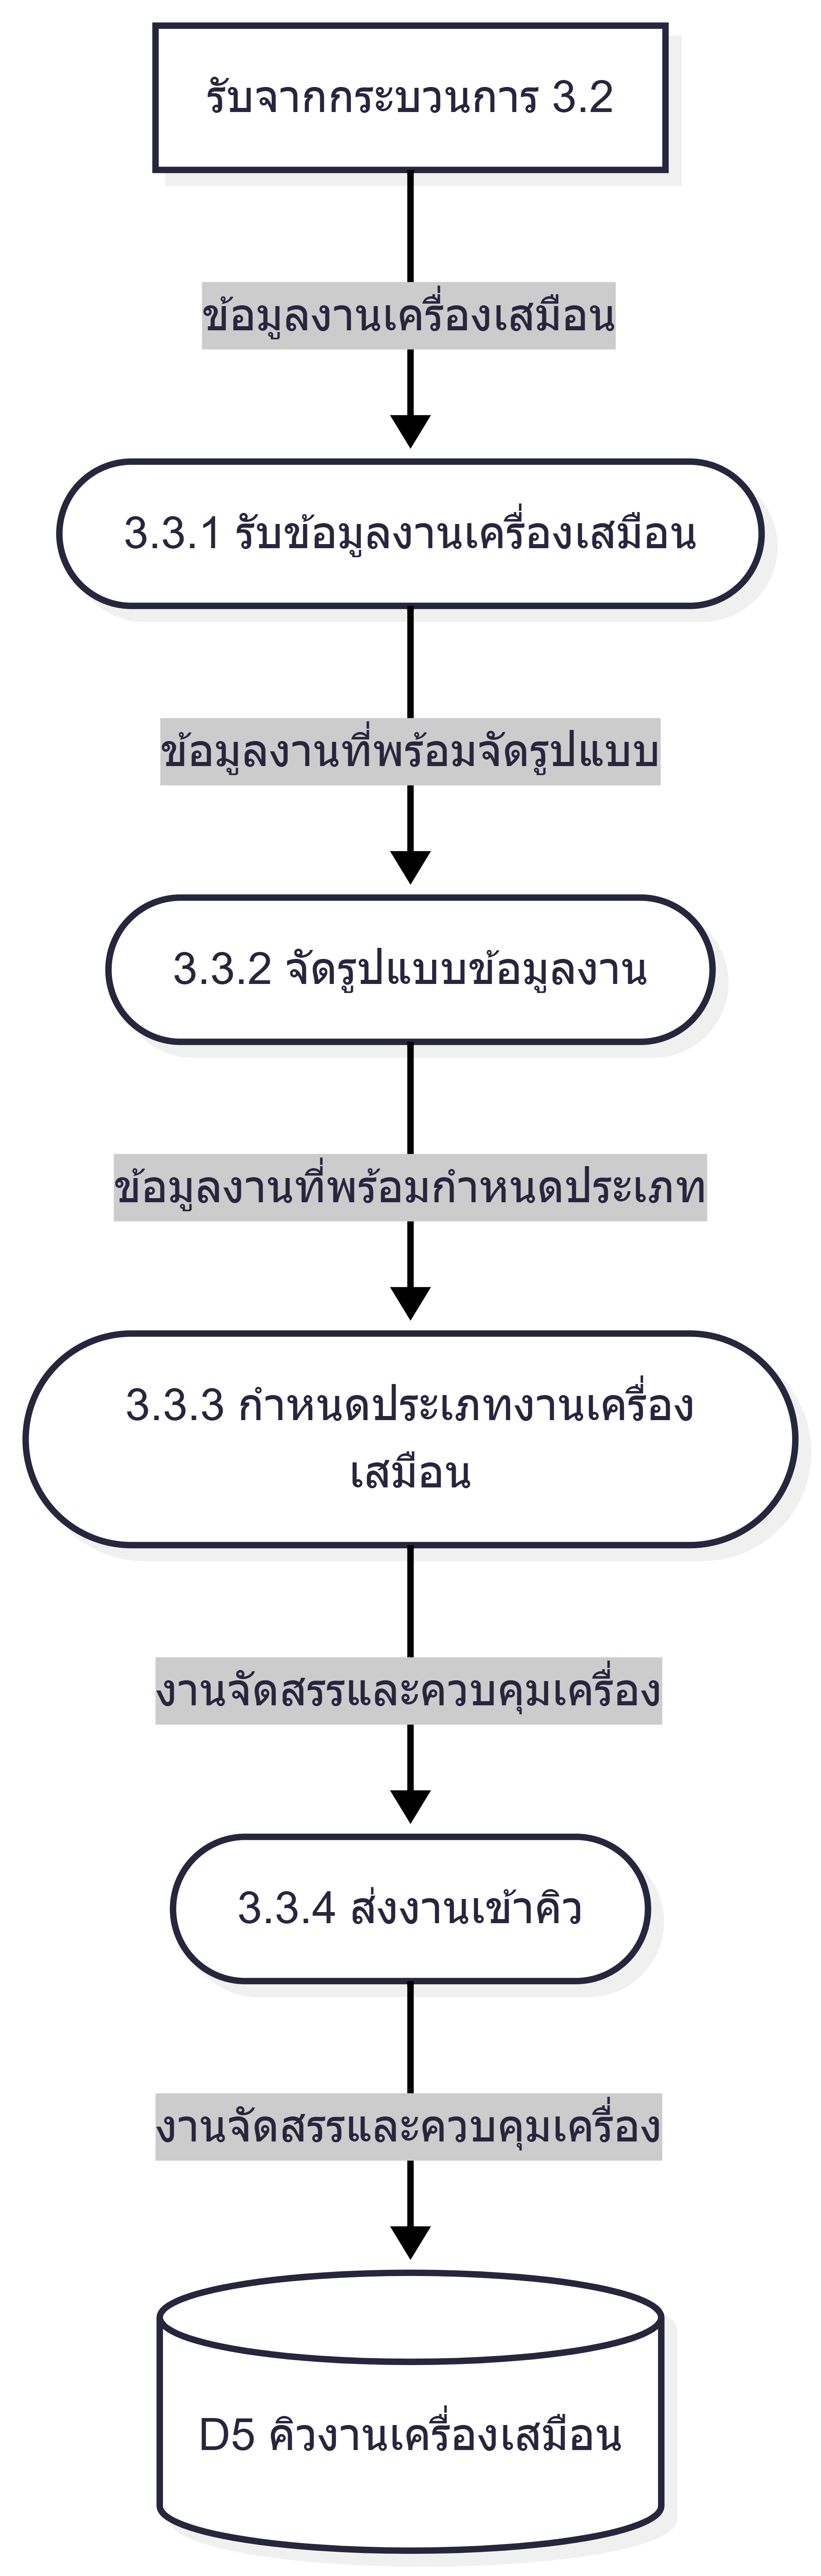
\includegraphics[width=0.35\textwidth]{Image/diagram/chapter3-dataflow-level2-process3-3.png}
    \caption{\fontSixTeen{แผนภาพการไหลของข้อมูลระดับที่ 2 ของกระบวนการ 3.3 การส่งงานเข้าคิว}}
    \label{fig3:data_flow_level_2_queue}
\end{figure}

\hspace*{1.3em} %ย่อหน้า
\textbf{กระบวนการ 3.3 การส่งงานเข้าคิว} (ภาพที่ \ref{fig3:data_flow_level_2_queue}) ระบบจะสร้าง payload ของงานโดยเก็บเฉพาะตัวระบุ (เช่น instanceId, userId, action) และข้อมูลที่จำเป็นขั้นต่ำ เพื่อหลีกเลี่ยงข้อมูลซ้ำซ้อนหรือข้อมูลล้าสมัยในคิว จากนั้นจึงส่งงานเข้าสู่ Redis-backed BullMQ พร้อมกำหนดชนิดงาน (เช่น provision/deprovision/toggle status) และอัปเดตสถานะงานในฐานข้อมูลเพื่อสะท้อนว่าอยู่ระหว่างรอประมวลผล วิธีนี้ช่วยให้การ retry มีความปลอดภัย เพราะ worker สามารถอ่านข้อมูลฉบับล่าสุดจากฐานข้อมูลก่อนลงมือปฏิบัติจริง

\begin{figure}[H]
    \centering
    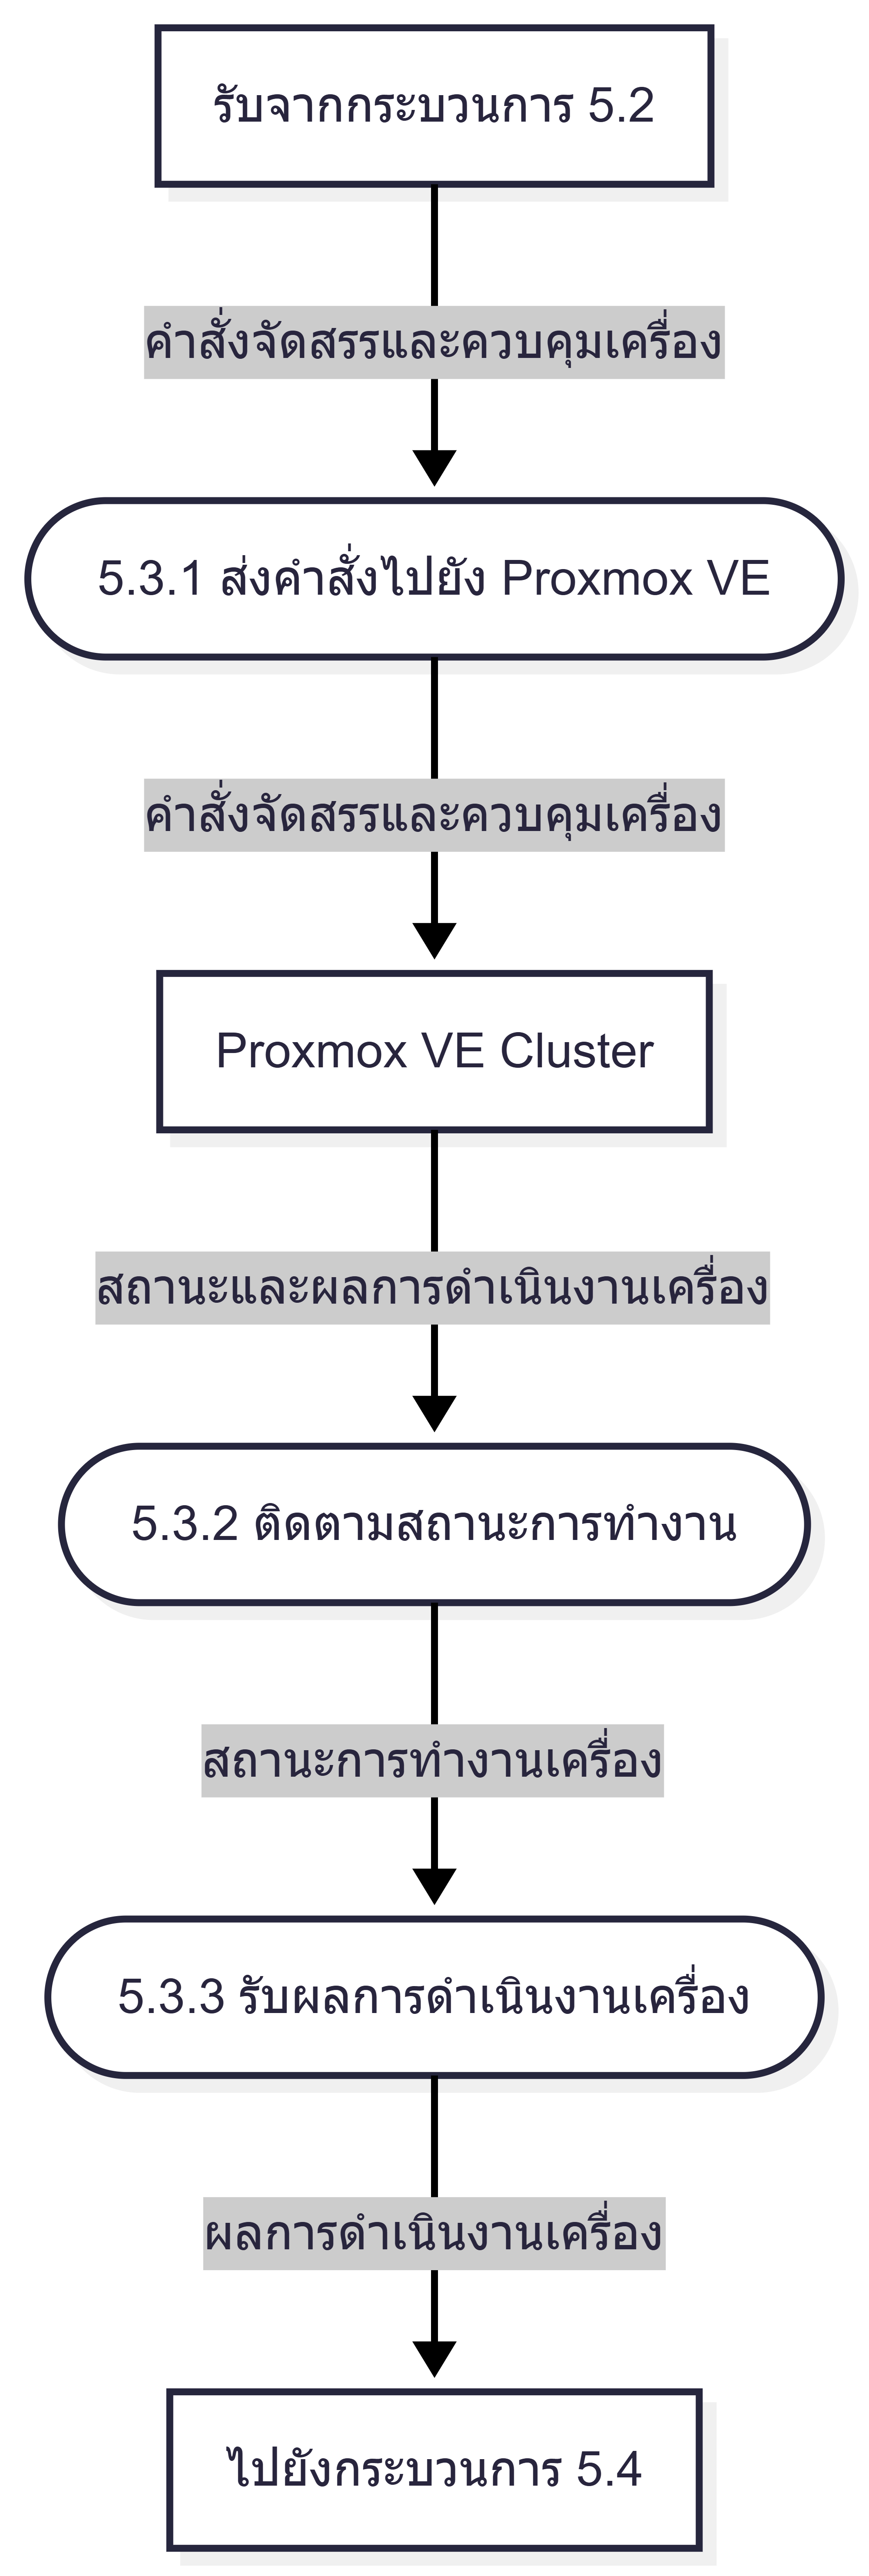
\includegraphics[width=0.35\textwidth]{Image/diagram/chapter3-dataflow-level2-process5-3.png}
    \caption{\fontSixTeen{แผนภาพการไหลของข้อมูลระดับที่ 2 ของกระบวนการ 5.3 การดำเนินการบน Proxmox VE}}
    \label{fig3:data_flow_level_2_pve}
\end{figure}

\hspace*{1.3em} %ย่อหน้า
\textbf{กระบวนการ 5.3 การดำเนินการบน Proxmox VE} (ภาพที่ \ref{fig3:data_flow_level_2_pve}) เริ่มจาก worker (Yuzu) รับงานจากคิวและโหลดรายละเอียด instance จากฐานข้อมูลเพื่อประกอบคำสั่ง จากนั้นเรียก Proxmox VE API เพื่อดำเนินการตามชนิดงาน (สร้าง/ลบ/เริ่ม/หยุด/รีสตาร์ท) พร้อมตรวจสอบผลลัพธ์และบันทึกสถานะงานเป็นช่วง ๆ หากเกิดข้อผิดพลาด worker จะบันทึกเหตุการณ์และสถานะล้มเหลวเพื่อให้ระบบแจ้งกลับผู้ใช้ได้อย่างถูกต้อง และหากเป็นกรณีที่รองรับการ retry จะสามารถหยิบงานขึ้นมาทำซ้ำได้โดยอ้างอิงสถานะล่าสุดในฐานข้อมูลเพื่อหลีกเลี่ยงการสร้าง VM ซ้ำหรือเปลี่ยนสถานะผิดพลาด

\newpage
\subsection{การออกแบบหน้าจอการทำงาน}
\hspace*{1.3em} %ย่อหน้า
การออกแบบหน้าจอการทำงานของระบบแพลตฟอร์มคลัสเตอร์เสมือนได้รับการออกแบบให้มีความสะดวกในการใช้งานและการเข้าถึงข้อมูลที่จำเป็น โดยแบ่งออกเป็นหน้าจอหลัก ๆ ดังนี้
\begin{mycustomitem}
    \item \textbf{หน้าจอเข้าสู่ระบบ (Login Page)} หน้าจอสำหรับผู้ใช้ในการเข้าสู่ระบบผ่านการยืนยันตัวตน
    \item \textbf{หน้าจอแดชบอร์ด (Dashboard)} แสดงภาพรวมสถานะเครื่องเสมือน รายการคำร้องขอ และข้อมูลผู้ใช้
    \item \textbf{หน้าจอจัดการเครื่องเสมือน (Instance Management)} สำหรับผู้ใช้ในการดูรายละเอียดเครื่องเสมือน เช่น สถานะ การเชื่อมต่อ และการจัดการเครื่อง
    \item \textbf{หน้าจอคำร้องขอเครื่องเสมือน (Instance Request)} สำหรับผู้ใช้ในการส่งคำร้องขอการใช้งานเครื่องเสมือน
    \item \textbf{หน้าจอจัดการคำร้องขอ (Request Management)} สำหรับเจ้าหน้าที่ในการตรวจสอบและอนุมัติคำร้องขอเครื่องเสมือน
\end{mycustomitem}
โดยมีการออกแบบหน้าจอหลัก ๆ ดังแสดงในภาพที่ \ref{fig3:login_page} – \ref{fig3:request_management}

\begin{figure}[H]
    \centering
    \fbox{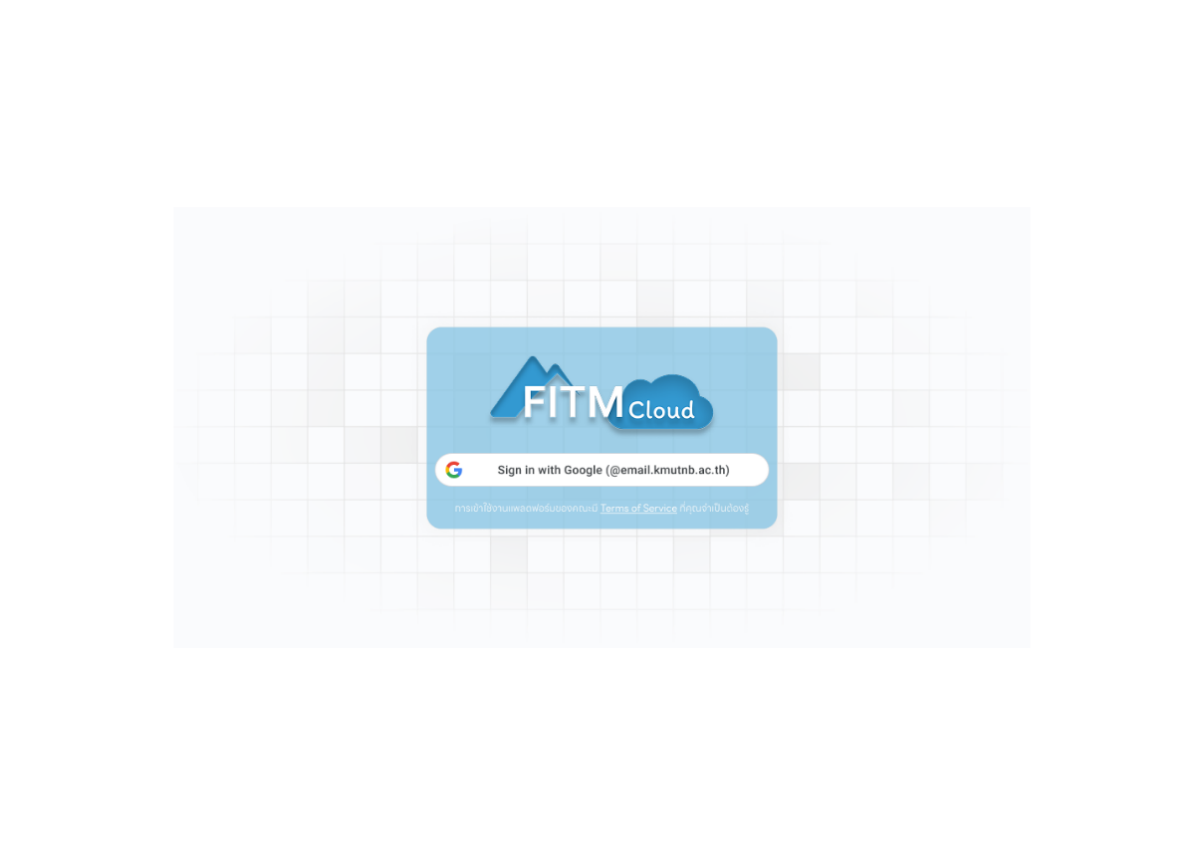
\includegraphics[width=0.9\textwidth]{Image/design/image2.png}}
    \caption{\fontSixTeen{หน้าจอเข้าสู่ระบบ (Login Page)}}
    \label{fig3:login_page}
\end{figure}

\begin{figure}[H]
    \centering
    \fbox{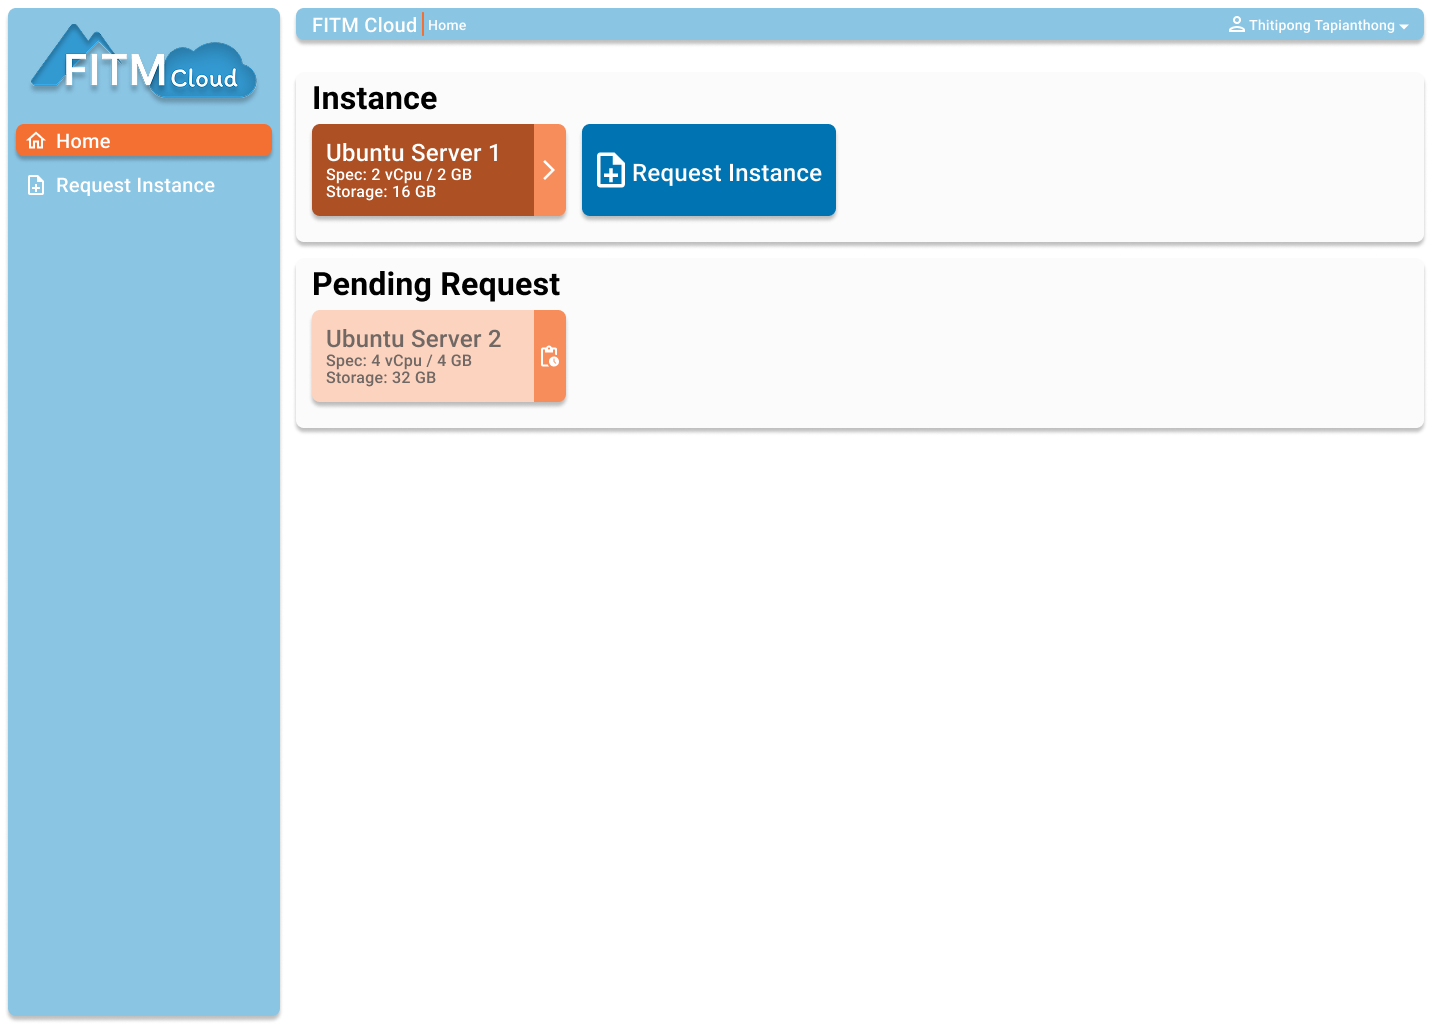
\includegraphics[width=0.9\textwidth]{Image/design/image3.png}}
    \caption{\fontSixTeen{หน้าจอแดชบอร์ด (Dashboard)}}
    \label{fig3:dashboard}
\end{figure}

\begin{figure}[H]
    \centering
    \fbox{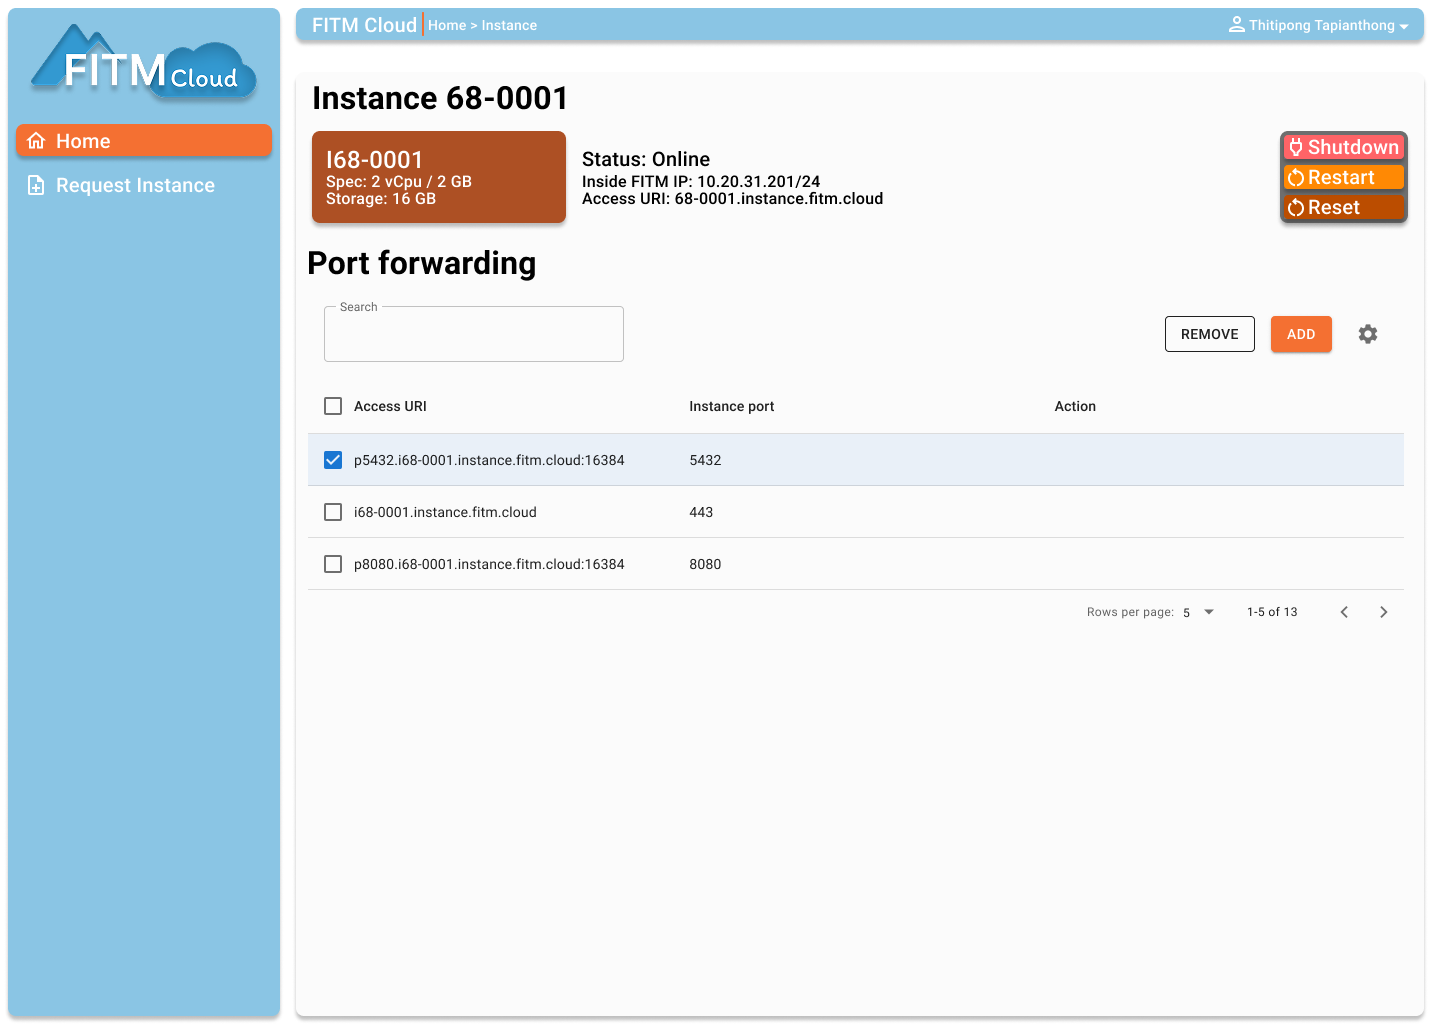
\includegraphics[width=0.9\textwidth]{Image/design/image5.png}}
    \caption{\fontSixTeen{หน้าจอจัดการเครื่องเสมือน (Instance Management)}}
    \label{fig3:instance_management}
\end{figure}

\begin{figure}[H]
    \centering
    \fbox{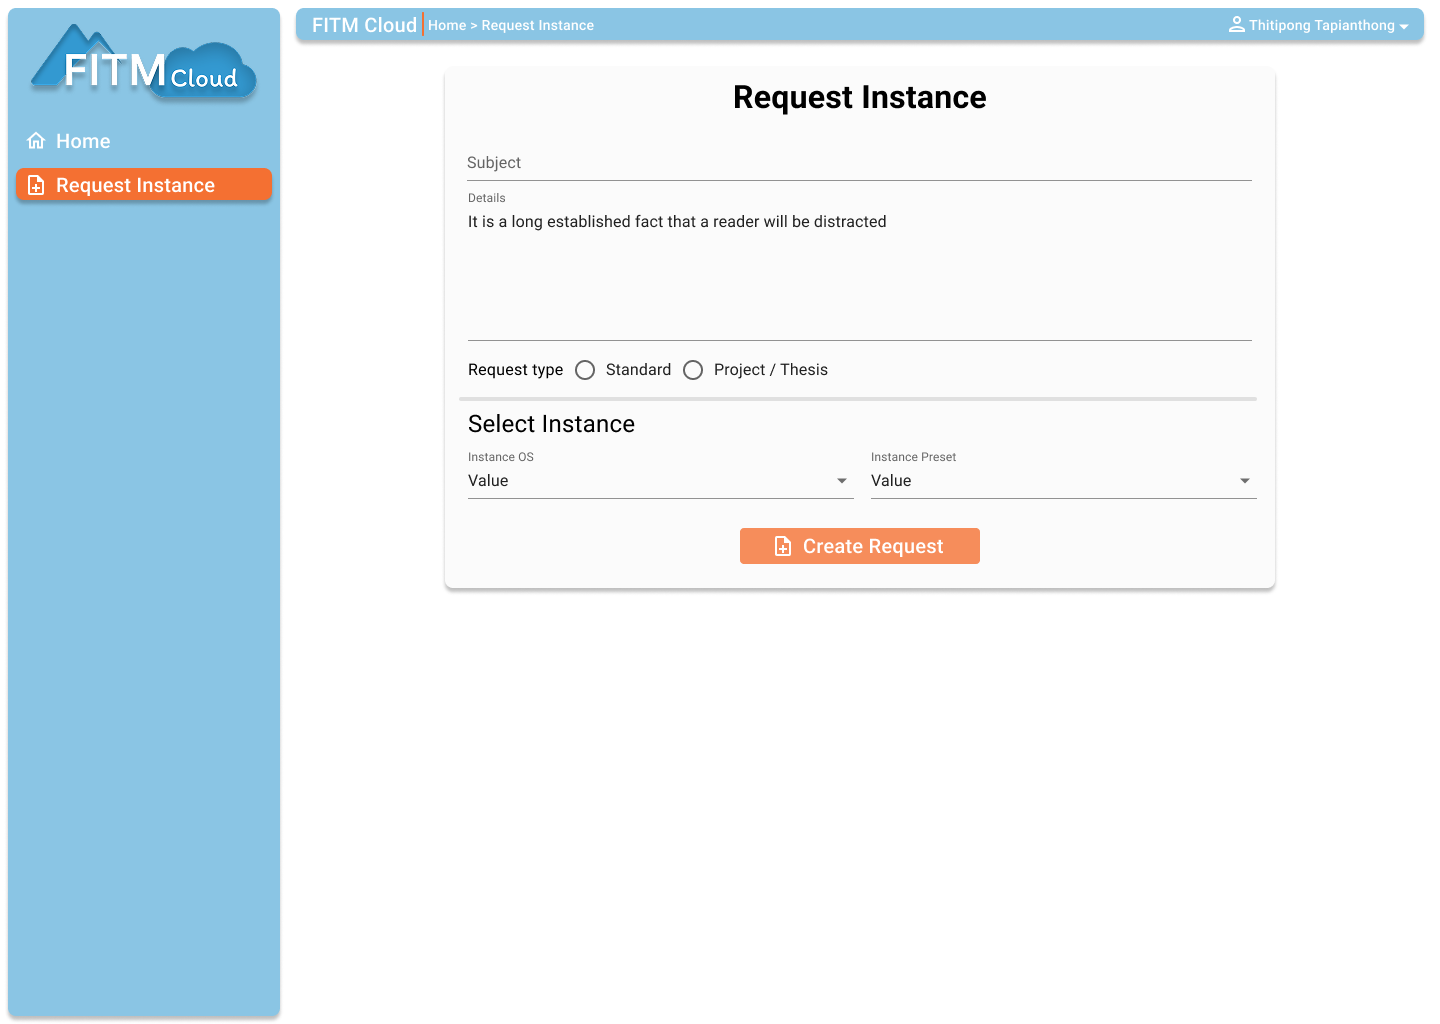
\includegraphics[width=0.9\textwidth]{Image/design/image4.png}}
    \caption{\fontSixTeen{หน้าจอคำร้องขอเครื่องเสมือน (Instance Request)}}
    \label{fig3:instance_request}
\end{figure}

\begin{figure}[H]
    \centering
    \fbox{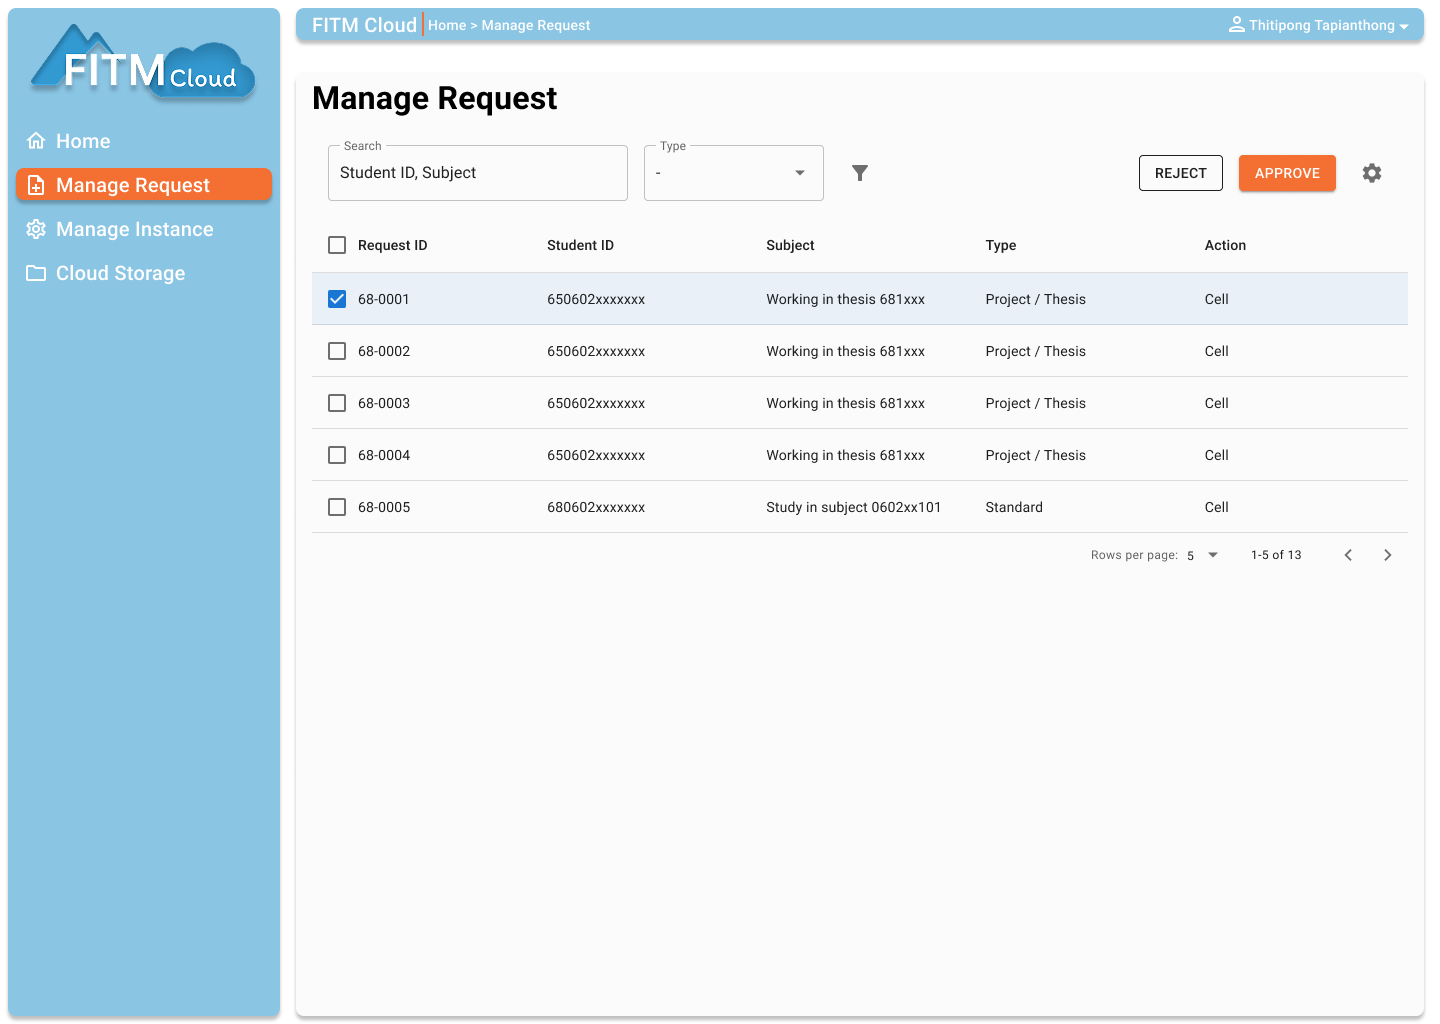
\includegraphics[width=0.9\textwidth]{Image/design/image7.png}}
    \caption{\fontSixTeen{หน้าจอจัดการคำร้องขอ (Request Management)}}
    \label{fig3:request_management}
\end{figure}

\newpage
% 3.3.2
\subsection{การออกแบบฐานข้อมูล}

\hspace*{1.3em} %ย่อหน้า
ระบบใช้ PostgreSQL เป็นฐานข้อมูลหลัก และใช้ Prisma ORM ในการกำหนดสคีมาและสร้างชั้นเข้าถึงข้อมูล โดยในฉบับพัฒนาปัจจุบันโครงสร้างฐานข้อมูลสามารถสรุปเป็นกลุ่มข้อมูลหลักดังนี้
\begin{mycustomitem}
    \item \textbf{Authentication and Role Management} เช่น User, Session, Account, Verification และ PlatformUser สำหรับจัดการตัวตนผู้ใช้งาน เซสชัน และบทบาท ADMIN, INSTRUCTOR, STUDENT
    \item \textbf{Academic Structure} เช่น Course, Semester, CourseOffering และ InstructorSearch สำหรับเชื่อมโยงรายวิชา ภาคการศึกษา และผู้สอน
    \item \textbf{Virtualization Resources} เช่น PVENode, PVENetwork, PVENetworkIP, PVETemplate และ PVEVM สำหรับสะท้อนทรัพยากรที่เกี่ยวข้องกับ Proxmox VE
    \item \textbf{Request Workflow} เช่น Request, ExtendedRequest, RequestAuditLog และ ExtendedRequestAuditLog สำหรับคำร้องขอเครื่องเสมือน การขยายสิทธิ์การใช้งาน และประวัติการอนุมัติ
    \item \textbf{Instance Management} เช่น Instance, InstanceReverseProxy, InstanceAuditLog และ PlatformSSHKey สำหรับข้อมูลเครื่องเสมือน ช่องทางการเชื่อมต่อ และบันทึกการเปลี่ยนแปลง
    \item \textbf{Platform Storage} เช่น PlatformFile สำหรับการจัดเก็บไฟล์
\end{mycustomitem}

% แผนภาพนี้ถูกสร้างจากไฟล์ Mermaid: docs/database/db-overview.mmd
\begin{figure}[H]
    \centering
    
\includegraphics[width=1.0\textwidth]{Image/diagram/database/db-overview.png}
    \caption{\fontSixTeen{แผนภาพโครงสร้างฐานข้อมูลของระบบภาพรวม (ER Diagram Overview)}}
    \label{fig3:database_schema}
\end{figure}

% แผนภาพนี้ถูกสร้างจากไฟล์ Mermaid: docs/database/db-auth.mmd
\begin{figure}[H]
    \centering
    
\includegraphics[width=1.0\textwidth]{Image/diagram/database/db-auth.png}
    \caption{\fontSixTeen{แผนภาพ ER กลุ่มข้อมูลการยืนยันตัวตนและผู้ใช้งาน}}
    \label{fig3:database_schema-1}
\end{figure}

% แผนภาพนี้ถูกสร้างจากไฟล์ Mermaid: docs/database/db-academic.mmd
\begin{figure}[H]
    \centering
    
\includegraphics[width=1.0\textwidth]{Image/diagram/database/db-academic.png}
    \caption{\fontSixTeen{แผนภาพ ER กลุ่มข้อมูลโครงสร้างวิชาการ}}
    \label{fig3:database_schema-2}
\end{figure}

% แผนภาพนี้ถูกสร้างจากไฟล์ Mermaid: docs/database/db-pve.mmd
\begin{figure}[H]
    \centering
    
\includegraphics[width=1.0\textwidth]{Image/diagram/database/db-pve.png}
    \caption{\fontSixTeen{แผนภาพ ER กลุ่มข้อมูลโครงสร้างพื้นฐาน Proxmox VE}}
    \label{fig3:database_schema-3}
\end{figure}

% แผนภาพนี้ถูกสร้างจากไฟล์ Mermaid: docs/database/db-instance.mmd
\begin{figure}[H]
    \centering
    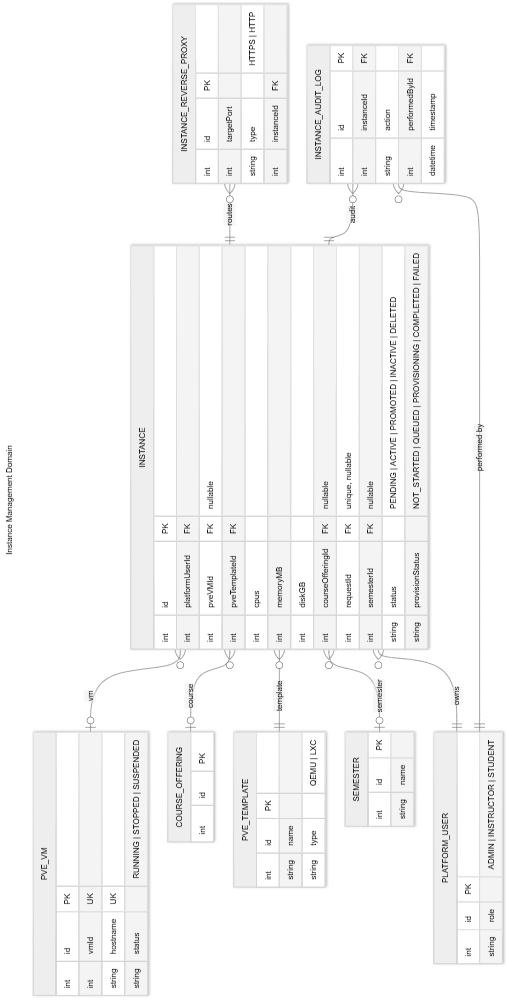
\includegraphics[width=0.75\textwidth]{Image/diagram/database/db-instance_90.png}
    \caption{\fontSixTeen{แผนภาพ ER กลุ่มข้อมูลการจัดการเครื่องเสมือน}}
    \label{fig3:database_schema-4}
\end{figure}

% แผนภาพนี้ถูกสร้างจากไฟล์ Mermaid: docs/database/db-request.mmd
\begin{figure}[H]
    \centering
    
\includegraphics[width=0.9\textwidth]{Image/diagram/database/db-request.png}
    \caption{\fontSixTeen{แผนภาพ ER กลุ่มข้อมูลคำร้องขอและกระบวนการอนุมัติ}}
    \label{fig3:database_schema-5}
\end{figure}

% แผนภาพนี้ถูกสร้างจากไฟล์ Mermaid: docs/database/db-storage.mmd
\begin{figure}[H]
    \centering
    
\includegraphics[width=0.75\textwidth]{Image/diagram/database/db-storage.png}
    \caption{\fontSixTeen{แผนภาพ ER กลุ่มข้อมูลพื้นที่จัดเก็บไฟล์}}
    \label{fig3:database_schema-6}
\end{figure}

\hspace*{1.3em} %ย่อหน้า
จากภาพที่ \ref{fig3:database_schema} – \ref{fig3:database_schema-6} จะเห็นได้ว่าการออกแบบฐานข้อมูลไม่ได้ครอบคลุมเฉพาะข้อมูลผู้ใช้และเครื่องเสมือนเท่านั้น แต่ยังรวมถึงโครงสร้างทางวิชาการ ประวัติการอนุมัติ การจัดการ reverse proxy และระบบจัดเก็บไฟล์ภายในแพลตฟอร์มด้วย ทั้งนี้ได้แบ่งแผนภาพเป็น 6 กลุ่มตามโดเมนข้อมูล ได้แก่ การยืนยันตัวตน โครงสร้างวิชาการ โครงสร้างพื้นฐาน Proxmox VE การจัดการเครื่องเสมือน กระบวนการคำร้องขอ และพื้นที่จัดเก็บไฟล์ การออกแบบในลักษณะนี้ทำให้ Momoi สามารถทำหน้าที่เป็นศูนย์กลางของข้อมูลธุรกรรม ขณะที่ Yuzu ใช้ข้อมูลเดียวกันในการอ้างอิงระหว่างการประมวลผลคำสั่งบน Proxmox VE

\begin{table}[H]
    \caption{\fontSixTeen{สรุปกลุ่มข้อมูลหลักจาก Prisma Schema ฉบับปัจจุบัน}}\label{tab3:db_domain_overview}
    \fontSixTeen
    \renewcommand{\arraystretch}{1.2}
    \begin{tabularx}{\textwidth}{|L|X|}
        \hline
	        \textbf{กลุ่มข้อมูล} & \multicolumn{1}{|>{\centering\arraybackslash}X|}{\textbf{เอนทิตีหลัก}} \\
        \hline
        Authentication และ RBAC & User, Session, Account, Verification, PlatformUser \\
        โครงสร้างวิชาการ & Course, Semester, CourseOffering, InstructorSearch \\
        ทรัพยากร Proxmox VE & PVENode, PVENetwork, PVENetworkIP, PVETemplate, PVEVM \\
        กระบวนการคำร้องขอ & Request, ExtendedRequest, RequestAuditLog, ExtendedRequestAuditLog \\
        การจัดการเครื่องเสมือน & Instance, InstanceReverseProxy, InstanceAuditLog, PlatformSSHKey \\
        พื้นที่จัดเก็บไฟล์ & PlatformFile \\
        \hline
    \end{tabularx}
\end{table}

\begin{table}[H]
    \caption{\fontSixTeen{รายการ Enum สำคัญในสคีมาฐานข้อมูลฉบับปัจจุบัน}}\label{tab3:db_enums_current}
    \fontSixTeen
    \renewcommand{\arraystretch}{1.2}
    \begin{tabularx}{\textwidth}{|l|L|}
        \hline
	        \textbf{ชื่อ Enum} & \multicolumn{1}{|>{\centering\arraybackslash}X|}{\textbf{ค่า}} \\
        \hline
        PlatformRole & ADMIN, INSTRUCTOR, STUDENT \\
        PVEVMStatus & RUNNING, STOPPED, SUSPENDED \\
        PVEVMType & QEMU, LXC \\
        InstanceStatus & PENDING, ACTIVE, PROMOTED, INACTIVE, DELETED \\
        InstanceProvisionStatus & NOT\_STARTED, QUEUED, PROVISIONING, COMPLETED, FAILED \\
        ReverseProxyType & HTTPS, HTTP \\
        ApprovalStatus & PENDING, APPROVED, REJECTED, CANCELLED \\
        \hline
    \end{tabularx}
\end{table}

% 3.3.3
\subsection{การออกแบบ API และการสื่อสาร}

\hspace*{1.3em} %ย่อหน้า
ระบบใช้ RESTful API เป็นหลักในการสื่อสารระหว่างส่วนประกอบ โดยมีการออกแบบดังนี้
\begin{mycustomitem}
    \item \textbf{Authentication Endpoints} ให้บริการผ่านเส้นทาง `/api/auth` โดย Momoi เป็นผู้ดูแลการยืนยันตัวตน Session และ OAuth callback ขณะที่ Midori จะใช้งานเส้นทางดังกล่าวผ่าน better-auth client
    \item \textbf{Platform API Endpoints} ให้บริการโดย Momoi ครอบคลุมโดเมนหลัก เช่น Academic Management, Request Workflow, Instance Management, Reverse Proxy Management และ Storage Management
    \item \textbf{Documentation and Telemetry Endpoints} ใช้สำหรับสร้าง OpenAPI Documentation, Metrics และ Traces เพื่อสนับสนุนการทดสอบและการติดตามสถานะของระบบ โดยกระจายอยู่ตามบทบาทของแต่ละบริการ
\end{mycustomitem}

\hspace*{1.3em} %ย่อหน้า
ตารางที่ \ref{tab3:api_groups} สรุปกลุ่ม API หลักของ Momoi พร้อมระดับการยืนยันตัวตนที่ต้องการ โดย Momoi เปิดเผย API ด้านแพลตฟอร์มเหล่านี้ผ่าน Elysia.js ซึ่งสร้าง OpenAPI Specification โดยอัตโนมัติ ทำให้ Midori สามารถนำข้อมูล Schema ไปสร้างชนิดข้อมูลฝั่ง Client ได้โดยตรงโดยไม่ต้องเขียนซ้ำ

\begin{table}[H]
    \caption{\fontSixTeen{สรุปกลุ่ม API หลักของบริการ Momoi}}\label{tab3:api_groups}
    \fontSixTeen
    \renewcommand{\arraystretch}{1.2}
    \begin{tabularx}{\textwidth}{|l|X|}
        \hline
        \textbf{กลุ่ม API} & \multicolumn{1}{|>{\centering\arraybackslash}X|}{\textbf{คำอธิบาย}} \\
        \hline
        Public & ข้อมูลสาธารณะ เช่น ภาคการศึกษาปัจจุบันและที่กำลังจะมาถึง \\
        Auth & Login, Logout, Session, OAuth callback \\
        Academic & รายวิชา ภาคการศึกษา ผู้สอน และการเปิดสอน \\
        Request & สร้างและจัดการคำร้องขอเครื่องเสมือน ทั้ง Request และ ExtendedRequest \\
        Instance & เครื่องเสมือน Reverse Proxy Audit Log และ SSH Key \\
        Storage & ไฟล์ โฟลเดอร์ การแบ่งปัน และสิทธิ์การเข้าถึง \\
        Admin & จัดการ PVE Node PVE Template PVE Network และ Platform User \\
        \hline
    \end{tabularx}
\end{table}

\hspace*{1.3em} %ย่อหน้า
การยืนยันตัวตนของระบบออกแบบให้ใช้ Session ผ่านชุด endpoint `/api/auth` ซึ่งใช้ `better-auth` และข้อมูลผู้ใช้ในฐานข้อมูลร่วมกัน จากนั้นเมื่อ Midori เรียก API ของ Momoi ต่อไป Momoi จะตรวจสอบ session และดึงข้อมูล PlatformUser จากฐานข้อมูลเพื่อกำหนดบทบาท (ADMIN, INSTRUCTOR, STUDENT) ก่อนอนุมัติคำขอ แนวทางนี้ทำให้การยืนยันตัวตนและการกำหนดสิทธิ์เชื่อมต่อกับ business logic ของแพลตฟอร์มได้โดยตรง และลดความซับซ้อนของ topology ที่ต้องติดตามในเอกสารและการติดตั้งใช้งาน

% 3.3.4
\subsection{การออกแบบระบบ Message Queue}

\hspace*{1.3em} %ย่อหน้า
ระบบรองรับการประมวลผลแบบ Asynchronous โดยใช้ Redis ร่วมกับ BullMQ เป็นกลไก Message Queue ระหว่าง Momoi และ Yuzu คิวหลักในฉบับพัฒนาปัจจุบันประกอบด้วย
\begin{mycustomitem}
    \item \textbf{Provision Queue} สำหรับงานสร้างและจัดสรรเครื่องเสมือนใหม่
    \item \textbf{Deprovision Queue} สำหรับงานลบหรือคืนทรัพยากรของเครื่องเสมือน
    \item \textbf{Toggle Status Queue} สำหรับงานเปลี่ยนสถานะของเครื่อง เช่น Start, Stop และ Restart
\end{mycustomitem}

\hspace*{1.3em} %ย่อหน้า
ในระดับการติดตั้งใช้งานจริง คิวเหล่านี้จะถูกตั้งชื่อแบบผูกกับ environment นำหน้าชื่อคิวเพื่อแยกงานของแต่ละสภาพแวดล้อมออกจากกันอย่างชัดเจน

\hspace*{1.3em} %ย่อหน้า
ข้อมูลที่ถูกส่งเข้าแต่ละงานจะเก็บเฉพาะตัวระบุที่จำเป็น เช่น `instanceId`, `userId` และ action ที่ต้องการเปลี่ยนแปลง จากนั้น Yuzu จะอ่านข้อมูลฉบับเต็มจากฐานข้อมูลก่อนดำเนินการบน Proxmox VE วิธีการนี้ช่วยลดความซ้ำซ้อนของข้อมูลในคิว ลดโอกาสใช้ข้อมูลที่ล้าสมัย และทำให้การ retry งานมีความปลอดภัยมากขึ้น

\hspace*{1.3em} %ย่อหน้า
ระบบกำหนดนโยบายการทำซ้ำงาน (retry policy) เพื่อรองรับความล้มเหลวชั่วคราว เช่น การเชื่อมต่อ Proxmox VE ขัดข้อง หรือ VM อยู่ระหว่างเปลี่ยนสถานะ โดยงานที่ล้มเหลวจะถูก retry ตามจำนวนครั้งที่กำหนด พร้อมการหน่วงเวลาแบบ exponential backoff ระหว่างครั้ง หากยังล้มเหลวเกินจำนวนที่กำหนดจะถูกย้ายเข้า failed job queue เพื่อให้ผู้ดูแลระบบตรวจสอบในภายหลัง ตารางที่ \ref{tab3:queue_jobs} สรุปคิวงานหลักพร้อมข้อมูลที่ส่งพร้อมแต่ละงานและผลลัพธ์ที่คาดหวัง

\begin{table}[H]
    \caption{\fontSixTeen{สรุปคิวงานหลักและโครงสร้างข้อมูลงาน}}\label{tab3:queue_jobs}
    \fontSixTeen
    \renewcommand{\arraystretch}{1.2}
    \begin{tabularx}{\textwidth}{|l|X|X|}
        \hline
        \textbf{ชื่อคิว} & \multicolumn{1}{|>{\centering\arraybackslash}X|}{\textbf{ข้อมูลหลักในงาน}} & \multicolumn{1}{|>{\centering\arraybackslash}X|}{\textbf{ผลลัพธ์ที่คาดหวัง}} \\
        \hline
        Provision & instanceId, userId & VM ถูกสร้างและพร้อมใช้งาน สถานะ Instance อัปเดตเป็น ACTIVE \\
        Deprovision & instanceId, userId & VM ถูกลบออกจากระบบ สถานะ Instance อัปเดตเป็น DELETED \\
        Toggle Status & instanceId, userId, action (START STOP RESTART) & สถานะ VM และ Instance ถูกอัปเดตให้สอดคล้องกับการสั่ง Start Stop หรือ Restart \\
        \hline
    \end{tabularx}
\end{table}

% Tools and Technologies Used
\section{เครื่องมือและเทคโนโลยีที่ใช้ในการพัฒนา}

% 3.4.1
\subsection{เทคโนโลยี Frontend}

\hspace*{1.3em} %ย่อหน้า
\textbf{Next.js 16 และ React 19} เป็นเทคโนโลยีหลักของส่วน Frontend เนื่องจากมีคุณสมบัติที่เหมาะสมกับการพัฒนาเว็บแอปพลิเคชันเชิงระบบดังนี้
\begin{mycustomitem}
    \item \textbf{App Router} สำหรับการจัดการ Routing แบบใหม่
    \item \textbf{Built-in TypeScript Support} รองรับ Type Safety
    \item \textbf{Integration with API Proxy and OpenAPI Types} ช่วยให้ส่วน Frontend สามารถเชื่อมต่อกับ Momoi ได้อย่างมีชนิดข้อมูลที่ชัดเจนและลดความซ้ำซ้อนของ schema ระหว่าง frontend กับ backend
\end{mycustomitem}

\hspace*{1.3em} %ย่อหน้า
\textbf{Tailwind CSS และชุดคอมโพเนนต์บน Radix UI} ใช้สำหรับการจัดการส่วนติดต่อผู้ใช้ เนื่องจาก
\begin{mycustomitem}
    \item \textbf{Utility-first} เขียน CSS ได้เร็วและมีประสิทธิภาพ
    \item \textbf{Responsive Design} รองรับการแสดงผลบนอุปกรณ์ต่าง ๆ
    \item \textbf{Composable UI Primitives} ช่วยให้สร้างฟอร์ม แดชบอร์ด และกล่องโต้ตอบที่ปรับใช้ซ้ำได้ง่าย
\end{mycustomitem}

% 3.4.2
\subsection{เทคโนโลยี Backend}

\hspace*{1.3em} %ย่อหน้า
\textbf{Elysia.js} เป็น Web Framework ที่ใช้กับ Bun Runtime โดยมีเหตุผลในการเลือกใช้ดังนี้
\begin{mycustomitem}
    \item \textbf{High Performance} มีประสิทธิภาพสูงกว่า Node.js Framework ทั่วไป
    \item \textbf{Type Safety} รองรับ TypeScript แบบเต็มรูปแบบ
    \item \textbf{OpenAPI Integration} สร้าง API Documentation อัตโนมัติ
    \item \textbf{Observability Integration} รองรับการเชื่อมต่อกับ OpenTelemetry และการเก็บข้อมูลด้านประสิทธิภาพของบริการ
\end{mycustomitem}

\hspace*{1.3em} %ย่อหน้า
\textbf{Prisma ORM} ใช้สำหรับการจัดการฐานข้อมูล เนื่องจาก
\begin{mycustomitem}
    \item \textbf{Type-safe Database Client} ป้องกันข้อผิดพลาดในการเขียน Query
    \item \textbf{Database Migrations} จัดการการเปลี่ยนแปลง Schema อย่างเป็นระบบ
    \item \textbf{Centralized Domain Model} ช่วยให้สคีมาของข้อมูลด้านผู้ใช้ คำร้อง เครื่องเสมือน และพื้นที่จัดเก็บอยู่ในรูปแบบเดียวกัน
\end{mycustomitem}

% 3.4.3
\subsection{Infrastructure และ DevOps}

\hspace*{1.3em} %ย่อหน้า
\textbf{Docker} ใช้สำหรับการ Containerization ของแอปพลิเคชันและบริการสนับสนุน เพื่อ
\begin{mycustomitem}
    \item \textbf{Environment Consistency} สภาพแวดล้อมการพัฒนาและ Production เหมือนกัน
    \item \textbf{Easy Deployment} ง่ายต่อการ Deploy และ Scale
    \item \textbf{Resource Isolation} แยกทรัพยากรระหว่างแอปพลิเคชัน
\end{mycustomitem}

\hspace*{1.3em} %ย่อหน้า
\textbf{Docker Compose และ Kubernetes Manifests} ใช้สำหรับการจัดการ Multi-container Application และสภาพแวดล้อมการติดตั้งจริง
\begin{mycustomitem}
    \item \textbf{Service Orchestration} จัดการการเริ่มต้นและหยุดทำงานของ Service
    \item \textbf{Network Management} จัดการเครือข่ายระหว่าง Container
    \item \textbf{Volume Management} จัดการการแชร์ข้อมูลระหว่าง Container
    \item \textbf{Platform Deployment} กำหนดการติดตั้งบริการหลัก เช่น PostgreSQL, Redis, RustFS และชุดระบบสังเกตการณ์การทำงาน
\end{mycustomitem}

\hspace*{1.3em} %ย่อหน้า
\textbf{Observability Stack} ถูกนำมาใช้เพื่อวัดผลและติดตามสภาวะของระบบอย่างต่อเนื่อง
\begin{mycustomitem}
    \item \textbf{Prometheus} สำหรับเก็บ Metrics จากแต่ละบริการ
    \item \textbf{Grafana} สำหรับแสดง Dashboard และภาพรวมของระบบ
    \item \textbf{Loki และ Jaeger} สำหรับเก็บ Logs และ Traces
    \item \textbf{InfluxDB และ Exporters} สำหรับรองรับข้อมูลเชิงสังเกตการณ์เพิ่มเติมในระดับโครงสร้างพื้นฐาน
\end{mycustomitem}

% 3.4.4
\subsection{เครื่องมือการพัฒนา}

\hspace*{1.3em} %ย่อหน้า
\textbf{Version Control และ Collaboration}
\begin{mycustomitem}
    \item \textbf{Git} สำหรับการควบคุมเวอร์ชันของโค้ด
    \item \textbf{GitHub} สำหรับการเก็บโค้ดและการทำงานร่วมกัน
    \item \textbf{GitHub Actions} สำหรับ CI/CD Pipeline
\end{mycustomitem}

\hspace*{1.3em} %ย่อหน้า
\textbf{Code Quality และ Testing}
\begin{mycustomitem}
    \item \textbf{TypeScript-first Development} สำหรับ Static Type Checking ตลอดทุกบริการ
    \item \textbf{OpenAPI Code Generation} สำหรับสร้างชนิดข้อมูลและลดความคลาดเคลื่อนระหว่าง Frontend กับ Backend
    \item \textbf{Repository-specific Linting and Formatting} ใช้เครื่องมือที่เหมาะสมกับแต่ละบริการเพื่อควบคุมคุณภาพของโค้ดก่อนนำขึ้นใช้งาน
\end{mycustomitem}
